% Vorlage für eine Bachelorarbeit - 2012-2013 Timo Bingmann

% Dies ist nur eine Vorlage. Strikte Vorgaben wie die Bachelorarbeit auszusehen
% hat gibt es nicht. Darum können auch alle Teile angepasst werden.

% TODO: change away from the enabledeprecatedfontcommands
\documentclass[enabledeprecatedfontcommands,12pt,a4paper,twoside]{scrartcl}

% Diese (und weitere) Eingabedateien sind in UTF-8
\usepackage[utf8]{inputenc}

% Verwende gute Type 1 Font: Latin Modern
\usepackage[T1]{fontenc}
\usepackage{lmodern}

% Sprache des Dokuments (für Silbentrennung und mehr)
\usepackage[german,english]{babel}

% Seitengröße - verwende fast die ganze A4 Seite
\usepackage[tmargin=22mm,bmargin=22mm,lmargin=20mm,rmargin=20mm]{geometry}

% Einrückung und Abstand zwischen Paragraphen
\setlength\parskip{\smallskipamount}
\setlength\parindent{0pt}

% Einige Standard-Mathematik Pakete
\usepackage{latexsym,amsmath,amssymb,mathtools,textcomp}

% Unterstützung für Sätze und Definitionen
\usepackage{amsthm}

\newtheorem{Satz}{Satz}[section]
\newtheorem{Definition}[Satz]{Definition}
\newtheorem{Lemma}[Satz]{Lemma}

\numberwithin{equation}{section}

% Deutsches Literaturverzeichnis
\usepackage{bibgerm}

% Unterstützung zum Einbinden von Graphiken
\usepackage{graphicx}

% Pakete die tabular und array verbessern
\usepackage{array,multirow}

% Kleiner enumerate und itemize Umgebungen
\usepackage{enumitem}

\setlist[enumerate]{topsep=0pt}
\setlist[itemize]{topsep=0pt}
\setlist[description]{font=\normalfont,topsep=0pt}

\setlist[enumerate,1]{label=(\roman*)}

% TikZ für Graphiken in LaTeX
\usepackage{tikz}
\usetikzlibrary{calc}

% Aktuelle Section und Untersection am Seitenkopf
\usepackage{fancyhdr}

\fancypagestyle{plain}{
  \fancyhead{}
  \fancyfoot{}
  \fancyfoot[LE,RO]{\normalsize\thepage}
  \renewcommand{\headrulewidth}{0pt}
  \renewcommand{\footrulewidth}{0pt}
}

\fancypagestyle{normal}{
  \setlength{\headheight}{20pt}
  \setlength\footskip{32pt}
  \fancyhead{}
  \fancyhead[LE]{\normalsize\textsc{\nouppercase{\leftmark}}}
  \fancyhead[RO]{\normalsize\textsc{\nouppercase{\rightmark}}}
  \fancyfoot{}
  \fancyfoot[LE,RO]{\normalsize\thepage}
  \renewcommand{\headrulewidth}{0.4pt}
  \renewcommand{\footrulewidth}{0pt}
}

% Hyperref für Hyperlink und Sprungtexte
\usepackage{xcolor,hyperref}

\hypersetup{
  pdftitle={Hier den Titel der Arbeit},
  pdfauthor={Hier den Author der Arbeit},
  pdfsubject={Stichworte, weiteres Stichwort},
  colorlinks=true,
  pdfborder={0 0 0},
  bookmarksopen=true,
  bookmarksopenlevel=1,
  bookmarksnumbered=true,
  linkcolor=blue!60!black,
  %linkcolor=black,
  citecolor=blue!60!black,
  urlcolor=blue!60!black,
  filecolor=green!60!black,
  pdfpagemode=UseNone,
  unicode=true,
}

% Paket zum Setzen von Algorithmen in Pseudocode mit kleinen Stilanpassungen
\usepackage[ruled,vlined,linesnumbered,norelsize]{algorithm2e}
\DontPrintSemicolon
\def\NlSty#1{\textnormal{\fontsize{8}{10}\selectfont{}#1}}
\SetKwSty{texttt}
\SetCommentSty{emph}
\def\listalgorithmcfname{Algorithmenverzeichnis}
\def\algorithmautorefname{Algorithmus}
\let\chapter=\section % repariert ein Problem mit algorithm2e

\DeclareOldFontCommand{\bf}{\normalfont\bfseries}{\mathbf}

\usepackage{todonotes}
\usepackage{comment}
\usepackage{algorithm2e}

\newtheorem{definition}{Definition}

\begin{document}

%%%%%%%%%%%%%%%%%%%%%%%%%%%%%%%%%%%%%%%%%%%%%%%%%%%%%%%%%%%%%%%%%%%%%%

\pagestyle{empty} % keine Seitenzahlen

% Titelblatt der Arbeit
\begin{titlepage}

  \begin{center}\large

    \quad\includegraphics[height=17mm]{kit_logo_de.pdf} \hfill
    \includegraphics[height=20mm]{grouplogo-algo-blue.pdf}\quad\null

    \vfill

    Bachelorarbeit
    \vspace*{2cm}

    {\bf\huge Malleable TOHTN Planning \\using CrowdHTN and Mallob \par}
    % Siehe auch oben die Felder pdftitle={}
    % mit \par am Ende stimmt der Zeilenabstand

    \vfill

    Niko Wilhelm

    \vspace*{15mm}

    Abgabedatum: 19.10.2012

    \vspace*{45mm}

    \begin{tabular}{rl}
      Betreuer: & Prof. Dr. Peter Sanders \\
      & M.Sc. Dominik Schreiber \\
    \end{tabular}
    
    \vspace*{10mm}

    Institut für Theoretische Informatik, Algorithmik \\
    Fakultät für Informatik \\
    Karlsruher Institut für Technologie

    % English:
    % Institute of Theoretical Informatics, Algorithmics \\
    % Department of Informatics \\
    % Karlsruhe Institute of Technology

    \vspace*{12mm}
  \end{center}

\end{titlepage}

%%%%%%%%%%%%%%%%%%%%%%%%%%%%%%%%%%%%%%%%%%%%%%%%%%%%%%%%%%%%%%%%%%%%%%

\vspace*{0pt}\vfill

\hrule\medskip

Hiermit versichere ich, dass ich diese Arbeit selbständig verfasst und keine anderen, als die angegebenen Quellen und Hilfsmittel benutzt, die wörtlich oder inhaltlich übernommenen Stellen als solche kenntlich gemacht und die Satzung des Karlsruher Instituts für Technologie zur Sicherung guter wissenschaftlicher Praxis in der jeweils gültigen Fassung beachtet habe.

\bigskip

\noindent
Karlsruhe, den \today

% Unterschrift (handgeschrieben)

\vspace*{5cm}

\clearpage

%%%%%%%%%%%%%%%%%%%%%%%%%%%%%%%%%%%%%%%%%%%%%%%%%%%%%%%%%%%%%%%%%%%%%%

\vspace*{0pt}\vfill

\selectlanguage{german}
\begin{abstract}
\centerline{\bf Zusammenfassung}

Hier die deutsche Zusammenfassung.

Ich bin Blindtext. Von Geburt an. Es hat lange gedauert, bis ich begriffen habe, was es bedeutet, ein blinder Text zu sein: Man macht keinen Sinn. Man wirkt hier und da aus dem Zusammenhang gerissen. Oft wird man gar nicht erst gelesen. Aber bin ich deshalb ein schlechter Text? Ich weiß, dass ich nie die Chance haben werde im Stern zu erscheinen. Aber bin ich darum weniger wichtig? Ich bin blind! Aber ich bin gerne Text. Und sollten Sie mich jetzt tatsächlich zu Ende lesen, dann habe ich etwas geschafft, was den meisten ,,normalen`` Texten nicht gelingt.

Ich bin Blindtext. Von Geburt an. Es hat lange gedauert, bis ich begriffen habe, was es bedeutet, ein blinder Text zu sein: Man macht keinen Sinn. Man wirkt hier und da aus dem Zusammenhang gerissen. Oft wird man gar nicht erst gelesen. Aber bin ich deshalb ein schlechter Text? Ich weiß, dass ich nie die Chance haben werde im Stern zu erscheinen. Aber bin ich darum weniger wichtig? Ich bin blind! Aber ich bin gerne Text.

\end{abstract}

\vfill

\selectlanguage{english}
\begin{abstract}
\centerline{\bf Abstract}

And here an English translation of the German abstract.

I'm blind text. From birth. It took a long time until I realized what it means to be random text: You make no sense. You stand here and there out of context. Frequently, they do not even read. But I have a bad copy? I know that I will never have the chance of appearing in the. But I'm any less important? I'm blind! But I like to text. And you should see me now actually over, then I have accomplished something that is not possible in most ``normal'' copies.

I'm blind text. From birth. It took a long time until I realized what it means to be random text: You make no sense. You stand here and there out of context. Frequently, they do not even read. But I have a bad copy? I know that I will never have the chance of appearing in the. But I'm any less important? I'm blind! But I like to text.

\end{abstract}
%\selectlanguage{english}

\vfill\vfill\vfill
\clearpage

%%%%%%%%%%%%%%%%%%%%%%%%%%%%%%%%%%%%%%%%%%%%%%%%%%%%%%%%%%%%%%%%%%%%%%

\vspace*{0pt}\vfill

\section*{Danksagungen}

Thanks to i10pc135 which suffered much to make the experimental evaluation possible.

\vfill\vfill\vfill
\clearpage

%%%%%%%%%%%%%%%%%%%%%%%%%%%%%%%%%%%%%%%%%%%%%%%%%%%%%%%%%%%%%%%%%%%%%%

\pagestyle{normal}
% markiere sections im Seitenkopf links und subsections rechts
\renewcommand\sectionmark[1]{\markboth{\thesection\quad\MakeUppercase{#1}}{\thesection\quad\MakeUppercase{#1}}}
\renewcommand\subsectionmark[1]{\markright{\thesubsection\quad\MakeUppercase{#1}}}

% Inhaltsverzeichnis
\tableofcontents

\clearpage

%%%%%%%%%%%%%%%%%%%%%%%%%%%%%%%%%%%%%%%%%%%%%%%%%%%%%%%%%%%%%%%%%%%%%%

\listoffigures
\listoftables
\listofalgorithms

\clearpage

%%%%%%%%%%%%%%%%%%%%%%%%%%%%%%%%%%%%%%%%%%%%%%%%%%%%%%%%%%%%%%%%%%%%%%

\section{Introduction}
\subsection{Motivation}
\todo{quote the malleability paper on how great the feature is}

\subsection{Research Goal}
- Provide a performant parallel TOHTN planner by improving upon the Crowd planner
- provide an efficient malleable TOHTN planner
	- first it needs to be correct and complete
- Provide integration of TOHTN into the Mallob malleable load balancer
- Compare performance of parallel to malleable TOHTN planning
- 
\subsection{Thesis Overview}


\section{Preliminaries}

\subsection{Planner Properties}
- soundness: all solutions we find are correct
- completeness: we always find a plan if it exists
- correctness: kinda obvious
- systematicity (\cite{holler2020htn}): for search we explore each search node at most once (Kambhampati, Knoblock, \& Yang, 1995) -> not a problem for TOHTN? check p.18 in holler2020 again
- optimality: shortest plan (few planners, Lilotane maybe?)

\subsection{(TO)HTN Formalism}
\label{prelim: formalism}
In this section we first define what HTN and TOHTN problems are from a formal perspective \ref{prelim: tohtn problems}. Afterwards we take a short look at the algorithmic worst case complexity of HTN and TOHTN planning \ref{prelim: tohtn complexity}. We conclude by taking a short look at how hierarchical and classical planning compare in \ref{prelim: planning differences} and present the way in which we visualize hierarchical problems in this work in \ref{prelim: graphic tohtn}.

\subsubsection{Defining (TO)HTN Planning Problems}
\label{prelim: tohtn problems}
Both HTN and TOHTN planning are based on decomposing a list of initial tasks down into smaller subtasks until those subtasks can be achieved by simple actions. A number of formalisms for HTN plannings exist \cite{georgievski2015htn, behnke2018tracking, schreiber2021lilotane}. These formalisms are similar but differ slightly to suit specific planning approaches. In this work, we will reuse the formalism we introduced in \cite{bretl2021parallel} which is built on the definition by \cite{georgievski2015htn}.

\begin{definition} % predicate
	A \textbf{predicate} consists of two parts. Firstly a predicate symbol $p \in \mathcal{P}$ where $\mathcal{P}$ is the finite set of predicate symbols. Secondly of a list of terms $\tau_1, \ldots, \tau_k$ where each term $\tau_i$ is either a constant symbol $c \in \mathcal{C}$, with $\mathcal{C}$ being the finite set of constant symbols, or a variable symbol $v \in \mathcal{V}$, where $\mathcal{V}$ is the infinite set of variable symbols. \\
	The set of all predicates is called $\mathcal{Q}$.
\end{definition}
With the definition of a predicate in place, we can then define a grounding as well as our world state.
\begin{definition} % grounding
	A \textbf{ground predicate} is a predicate where the terms contain no variable symbols or, in other words, a predicate that contains only constant symbols.
\end{definition}
\begin{definition} % state
	A \textbf{state} $s \in 2^{\mathcal{Q}}$ is a set of ground predicates for which we make the closed-world-assumption. Under the closed-world-assumption, only positive predicates are explicitly represented in $s$. All predicates not in $s$ are implicitly negative.
\end{definition}

\begin{definition} % primitive task/ action
	With $T_p$ the set of primitive task symbols, a \textbf{primitive task} $t_p$ is defined as a triple $t_p(\Tilde{t}_p (a_1, \ldots, a_k), pre(t_p), eff(t_p))$. $\Tilde{p} \in T_p$ is the task symbol, $a_1, \ldots, a_k \in \mathcal{C} \cup \mathcal{V}$ are the task arguments, $pre(t_p) \in 2^{\mathcal{P}}$ the preconditions and $eff(t_p) \in 2^{\mathcal{P}}$ the effects of the primitive task $t_p$. We further define the positive and negative preconditions of $t_p$ as $pre^+(t_p) := \{p \in pre(t_p) : p \text{ is positive}\}$ and $pre^-(t_p) := \{p \in pre(t_p) : p \text{ is negative}\}$. We define $eff^+(t_p)$ and $eff^-(t_p)$ analogously. \\
	We call a fully ground primitive task an \textbf{action}.
\end{definition}

As preconditions and effects may not be concerned with the whole world state the closed-world assumption does not apply to them. To any HTN instance we could create an equivalent one where each precondition and effect cares about the whole world state. This would be achieved by instantiating all the "don't care" terms in preconditions and effects with all possible combinations of predicates. Doing this would, however, come at the price of a huge blowup of our planning problem. \\

\begin{definition} % applicable, application
	An action $t_p$ is \textbf{applicable} in state $s$ if $pre^+(t_p) \subseteq s$ and $pre^-(t_p) \cap s = \emptyset$. The \textbf{application} of $t_p$ in state $s$ results in the new state $s' = (s \setminus eff^-(t_p)) \cup eff^+(t_p)$.
\end{definition}

\begin{definition} % compound task/ abstract task
	We define a \textbf{compound task} as $t_c = \Tilde{t}_c(a_1, \ldots, a_k)$, where $\Tilde{t_c} \in T_c$ is the task symbol from the finite set of compound task symbols $T_c$ and $a_1, \ldots, a_k$ are the task arguments.
\end{definition}
Primitive and compound tasks together form task networks. In places where both can be used, we will refer to them simply as tasks $t \in T$.

\begin{definition} % task network
	Let $T = T_p \bigcup T_c$ be a set of primitive and compound tasks. A task network is a tuple $\tau = (T, \psi)$ consisting of tasks $T$ and constraints $\psi$ between those tasks.
\end{definition}

\begin{definition} % method, reduction
	Let $M$ be a finite set of method symbols and $T = T_p \bigcup T_c$ a set of primitive and compound tasks. A \textbf{method} $m = (\Tilde{m}(a_1, \ldots, a_k), t_c, pre(m), subtasks(m), constraints(m))$ is a tuple consisting of the method symbol $\Tilde{m}$, the method arguments $a_1, \ldots, a_k$, the associated compound task $t_c \in T_c$ the method refers to, a set of preconditions $pre(m) \in 2^{\mathcal{P}}$, a set of tasks $subtasks(m) = \{t_1, \ldots, t_l\}, t_i \in T$ and a set of ordering constraints $c_1, \ldots, c_m$ defining relationships between the subtasks. Any arguments appearing in $t_c, pre(m), subtasks(m)$ must also appear in $a_1, \ldots, a_k$.\\
	In TOHTN planning, $constraints(m)$ is implicitly set s.t. the subtasks $t_1, \ldots, t_l$ are totally ordered. \\
	We call a fully ground method a \textbf{reduction}.
\end{definition}
Each method $m$ has exactly one associated compound task $t_c$. However, multiple methods $m_1, \ldots, m_k$ may be associated with a single compound task $t_c$. Additionally, while any arguments of $t_c$ must be present in $m$, the contrary is not true and $m$ may have arguments not present in $t_c$, i.e., $m$ is not fully determined by $t_c$. As a result, methods represent choice points both in the choice of method itself as well as through the argument instantiation. \\


\begin{definition} % resolving a compound task
	Let $\tau = (T, \psi)$ be a task network, $s$ a state, $m = (\Tilde(m)(a_1, \ldots, a_k), t_c, pre(m),$\\$ subtasks(m), constraints(m))$ be a method. $m$ \textbf{resolves} $\tau$ iff $t_c \in T$, the constraints in $\psi$ allow for $t_c$ to be resolved, $pre^+(m) \in s$ and $pre^-(m) \cap s = \emptyset$. \\
	Resolving a compound task $t \in T$ results in a new task network $\tau' = ((T \setminus t) \cup \{t : t \in subtasks(m)\}, \psi \cup constraints(m))$ and unchanged state $s$. \\
	Applying a primitive task results in a new task network $\tau' = (T \setminus t, \psi)$ in state $s'$ where the effects of $t$ have been applied to $s$. 
\end{definition}

\begin{definition} % HTN domain, HTN problem
	An \textbf{HTN domain} is a tuple $D = (V, C, P, T, M)$ consisting of finite sets variables $V$, constants $C$, predicates $P$, tasks $T$ and methods $M$. An \textbf{HTN problem} $\Pi = (D, s_0, \tau_0)$ consists of a domain $D$, an initial state $s_0$ and an initial task network $\tau_0$. \\
	If $subtasks(m)$ has a total order for all $m \in M$ and the tasks in $\tau_0$ are totally ordered, we speak of a \textbf{TOHTN domain} and \textbf{TOHTN problem}.
\end{definition}
It is possible to simplify the model s.t. $\tau_0$ always consists of only a single task with no constraints. We do this by inserting a new initial task $t_0$ and method $m_0$ with no arguments s.t. resolving $t_0$ via $m_0$ results in $\tau_0$. \\
Another way of viewing HTN problems is as AND/OR trees \cite{holler2021landmark} where tasks form OR-nodes where one of may methods is chosen and methods form AND-nodes, as all subtasks need to be resolved.

\subsubsection{Complexity of (TO)HTN planning}
\label{prelim: tohtn complexity}
The complexity of HTN and TOHTN planning has been studied in many papers. Here the problem PLANEXIST describes, whether for any given (TO)HTN instance a plan exists at all. It is not concerned with optimality. \\
Early on it was shown by \cite{erol1994htn} and \cite{erol1996complexity} that the complexity of hierarchical planning formalisms depends on things such as the existence and ordering of non-primitive tasks, whether a total order between tasks is imposed and whether variables are allowed. The combination of arbitrary non-primitive tasks, no total order imposed and allowing variables is what we talk about with HTN planning, the same combination but with a total order is what we mean with TOHTN planning. They showed that HTN planning is semi-decidable whereas TOHTN planning is decidable in D-EXPTIME while being EXPSPACE-hard. \\
We can see what D-EXPTIME means in practise when we consider the maximum size of a task network we need to consider. From \cite{behnke2018totsat} we know that if a solution to an HTN instance exists, it can be found within a maximum depth of $|T_c| \cdot(2 ^{|\mathcal{Q}|})^2$. Similarly, we see that a task network can have exponential width in it's depth. Consider for this an instance constructed such that each compound task has exactly two children and where primitive tasks are only occuring at the bottom most layer. Now each layer will be twice as wide as the one before, giving us exponential width. \\
Regarding the general relationship of hierarchical planning to complexity theory, \cite{erol1994htn} and \cite{erol1996complexity} showed early on that HTN instances can be used to simulate context-free languages. This was extended by \cite{holler2014language} who showed that TOHTN instances correspond exactly to context-free grammars. \\
In addition to planning itself, the problem of plan verification was studied. Here, \cite{behnke2015complexity} showed that plan verification is NP-complete, even under the assumption that not only the plan but also the decompositions leading to it are provided.
\begin{comment}
\cite{erol1994htn}
- complexity depends on
	1. existence/ ordering of non-primitive tasks in task networks
	2. total order (or not) of tasks
	3. whether variables are allowed
- general HTN planning (non-primitive tasks are allowed, no guaranteed total order, variables are allowed) -> undecidable
- TOHTN planning (variables allowed, arbitrary non-primitive tasks) -> D-EXPTIME, EXPSPACE-hard
 
- context free grammars play a role, can be simulated in HTN

\cite{erol1996complexity}
- undecidable for HTN, D-EXPTIME and PSPACE-hard for TOHTN

both: context-free grammars can be simulated by HTN, use primitive tasks as terminals, abstract tasks as non-terminals, methods as grammar rules

\cite{holler2014language}
- TOHTN planning problems correspond to context free grammars

\cite{behnke2015complexity}
- HTN plan verification is NP-complete
- this even holds if the list of decompositions is provided
\end{comment}

\subsubsection{Differences from other Kinds of Planning}
\label{prelim: planning differences}
\cite{nau2007current} creates a classification of planners into domain-specific, domain-independent and domain-configurable planners.
They argue that HTN planning falls under domain-configurable with the decompositions providing advice to the planner to gain efficiency.
\cite{holler2020htn} argue that HTN-planning is not simply a domain-configurable version of classical planning on the basis that \cite{erol1994htn, erol1996complexity} showed that HTN-planning is strictly more powerful compared to classical planning which is PSPACE-complete. \\
While we agree with \cite{holler2020htn}, one can still use HTN planning without using the full complexity of the model, using it instead to provide more efficient and guided versions of classical planning problems.

\subsubsection{Graphically Representing TOHTN Problems}
\label{prelim: graphic tohtn}
In the rest of this work we will sometimes represent the structure of TOHTN domains graphically. We will always use the same scheme which we explain here. In our visualization, we represent the structure of a domain as a series of methods. To the left we show the compound task, followed by the method itself on its right and followed again by the method subtasks in their fixed order. Compound tasks are always represented by green rounded squares and their name, methods by an arrow with the method name above and actions by blue rounded squares and their name.\\
A short example is shown in figure \ref{figure: prelim tohtn example}. It consists of one method, $m_1$ which resolves task $t_1$. The subtasks of $m_1$ are $t_2$, $a_1$ and $a_2$. $t_1$ and $t_2$ are compound tasks, $a_1$ and $a_2$ are actions.
\begin{figure}
	\caption{An example TOHTN domain}
	\label{figure: prelim tohtn example}
	\centering
	
\includegraphics[width=0.7\textwidth]{images/final/domain_example}
\end{figure}

\subsection{Techniques to solve TOHTN planning problems}
\label{prelim: techniques}
In this section, we will give an overview over the different techniques with which HTN problems can be solved. The HTN planners produced by researchers can be classified along two main axes:
\begin{itemize}
	\item the planning algorithm
	\item lifted vs grounded approaches
\end{itemize}
For the algorithms, the two main variations are translation-based algorithms that take an HTN instance and translate it into a problem in a simpler complexity class such as classical planning or SAT and search-based algorithms, that utilize techniques such as plan-space search and progression search. We will focus on progression search here, as it is the technique employed in our own planner, CrowdHTN. \\
After that we will have a short discussion on lifted versus grounded approaches which is largely independent of the search algorithm.
\begin{comment}
- multiple ways to solve HTN instances
- planners can be classified on two axis: the algorithm and lifted vs grounded
- in practise, most algorithms are based on translation to SAT or on search algorithms
- we will focus on search-based as we will see in later section \ref{prelim: crowdhtn} that this is what our own planner utilizes
\end{comment}

\subsection{Translation-based}
\label{prelim: translation based planners}
One of the main techniques employed in HTN planning is to find an efficient encoding into a simpler problem. Two such problems are classical planning (\cite{alford2016bound}) and propositional logic (SAT). While translation to SAT was already proposed in 1998 (\cite{mali1998encoding}), the first complete encoding without assumptions about the instance was publicized in 2018 (\cite{behnke2018totsat}). In recent years, SAT seems to be the most popular problem to translate an HTN instance into, utilized by planners such as totSAT (\cite{behnke2018totsat}, \cite{behnke2018tracking}), Tree-REX (\cite{schreiber2019tree}) and Lilotane (\cite{schreiber2021lilotane}). \\
As we have seen in the previous section \ref{prelim: tohtn complexity} on (TO)HTN complexity, (TO)HTN problems are in D-EXPTIME and undecidable respectively. Both classical planning and SAT are less powerful. As a result, HTN problems cannot be encoded and even for TOHTN problems we would suffer a blowup in the size of the instance. Instead, as noted in \cite{schreiber2019tree}, SAT-based planners tend to explore the set of potential hierarchies layer by layer, increasing the encoding size as they go. As a result, those SAT-based planners tend to have a BFS-like characteristic to their search.

\begin{comment}
- may translate to classical planning \cite{alford2016bound}
- SAT-based has been known since 1998 \cite{mali1998encoding}
- tend to explore the hierarchy layer-by-layer \cite{schreiber2019tree}
- this gives the search a BFS-like characteristic
- this is needed, as SAT is NP-complete compared to HTN which is undecidable and TOHTN which is in D-EXPTIME \ref{prelim: tohtn complexity}
- encoding the whole instance would be impossible in case of HTN and lead to blowup in instance size in case of TOHTN
- going bit by bit is done instead

- example planners are Tree-REX \cite{schreiber2019tree}, totSAT \cite{behnke2018totsat}, Lilotane \cite{schreiber2021lilotane}
\end{comment}

\subsubsection{Search-based}
\label{prelim: techniques search}
The second main category of techniques to solve HTN planning problems are search-based algorithms, such as plan space search and progression search. Plan space search searches the space of partial plans, where search nodes represent partial plans and edges represent plan refinements \cite{weld1994introduction}. \\
As progression search is both more prominent in current planners and our own planner, CrowdHTN, also utilizes it we will now focus on this paradigm according to \cite{holler2020htn}.
Progression search on the other hand generates plans in a forward way. Search nodes are represented as tuples $(tn, s)$ of open tasks $tn$ and world state $s$. It always chooses an open task that is currently unconstrained, i.e. has no unresolved predecessors under the ordering constraints, and resolves it. This allows the planner to update the world state as it goes along, as the sequence of actions from the start to the current point is known at each step of the search. This world state information can thus be used to guide the planner towards the goal. In case of TOHTN planning, the choice of the next unconstrained task becomes trivial, as there is always exactly one such task. Knowing the full world state gives progression search two main advantages over plan space search. First, it allows the planner to prune parts of the search space by immediately validating action and reduction preconditions against this world state. Second, it gives us maximum information to be used in heuristics that guide our search. \\
The progression search algorithm is given in pseudocode in algorithm \ref{algo: progression search}. As mentioned, line 6 becomes trivial for TOHTN planning and the loop from lines 7  to 16 is no loop, as there is always exactly one unconstrained task. Additionally, the location of our goal test can be moved around, depending on need. Performing the goal test upon popping a node is useful if we want to find optimal plans and our fringe data structure - and thus popping order - have a notion of node cost. Performing the goal test upon node creation allows us to terminate earlier. \\
Notable search-based planners are SHOP (\cite{nau1999shop}), HyperTensioN (\cite{magnaguagno2020hypertension}), PANDA (\cite{holler2020htn}) and our own planner CrowdHTN which will be presented in a later section \ref{prelim: crowdhtn}.
\begin{comment}
\cite{holler2020htn}
- progression search is one of the best known search algorithms
- generate plans in a forward way
- always resolve a task that has no more open predecessors with the ordering constraints (is called 'unconstrained task')
- own: for TOHTN: we always have exactly 1 task we want to process next!
- makes it trivial to find the next unconstrained task
- mentioned in the paper
- progression search planners always know the current (world) state, can use this information for heuristics, pruning etc

- other planners search partial plans but not in order, they thus cannot know the current world state
- perform goal test on popping: find optimal plan if popping order is informed by cost
- perform goal test before popping: explore fewer nodes

- Alford et al, 2012, Thm. 3 -> HTN problem is solvable <=> there is a solution in progression space

- parts of the search space will be searched more than once if no additional measures are taken
\end{comment}
\begin{algorithm}
	\caption{Classical Progression Search for HTN as introduced in \cite{holler2020htn}}
	\label{algo: progression search}
	$fringe \gets \{ (s_0, tn_I, \epsilon)\}$\;
	\While{$fringe \neq \emptyset$}{
		$n \gets fringe.pop()$\;
		\If{$n.isgoal$}{
			\textbf{return} $n$\;
		}
		$U \gets n.unconstrainedNodes$\;
		\For{$t \in U$}{
			\eIf{$isPrimitive(t)$}{
				\If{$isApplicable(t)$}{
					$n' \gets n.apply(t)$\;
					$fringe.add(n')$\;
				}
			}{
				\For{$m \in t.methods$}{
					$n' \gets n.decompose(t, m)$\;
					$fringe.add(n')$\;
				}
			}
		}
	}
\end{algorithm}

\subsubsection{Lifted and Ground HTN Planning}
As mentioned in section \ref{prelim: tohtn problems}, HTN instances are normally given in a lifted representation and can be ground, i.e. all variables are filled with all possible parameter combinations. Specifying the instance in a lifted fashion is done for ease of use, as it is a more compact representation and allows domains to be reused for different problems \cite{behnke2020succinct}. \\
The efficient grounding and pruning of HTN instances is an active field of research (\cite{ramoul2017grounding}, \cite{behnke2020succinct}). While it is an easier problem than HTN planning itself, it can take exponential time the ground instance may still be exponential in size compared to the lifted instance \cite{behnke2020succinct}. \\
Planners may choose to operate on either lifted or ground instances. A discussion on the trade-offs involved is found in \cite{schreiber2021lilotane}. We will reiterate the main advantage of each approach here. Grounded representations have more information available for pruning. As an example, while some parameter combinations in reductions may lead to a contradiction later on and can thus be pruned, not all such combinations may be invalid and thus the corresponding lifted method may not be prunable. Lifted representations on the other hand may be a lot more compact in practice. For example, our (TO)HTN instance may want us to choose any of $N$ trucks to transport a package from $A$ to $B$ where in practice the choice might not matter. Whereas a grounded representation will have to instantiate all operators concerning a truck $N$ times, a lifted operation will avoid this and only choose a truck ad-hoc. \\
The choice of grounded vs lifted representation is independent of the choice of planning algorithm. We have examples of grounded translation-based planners (totSat \cite{behnke2018totsat}, Tree-REX \cite{schreiber2019tree}), lifted translation-based planners (Lilotane \cite{schreiber2021lilotane}) and also search-based planners that work on both lifted (HyperTensioN \cite{magnaguagno2020hypertension}) and ground representations (PANDA \cite{holler2020htn}). \\
Our own planner, CrowdHTN, walks a middle ground. It performs its search on a ground representation to allow detailed pruning according to the world state. However, it does not front-load the cost of a grounding procedure and instead grounds tasks and methods as needed.
\begin{comment}
- grounding can be an expensive operation \cite{behnke2020succinct}
- grounding is an active field of research within hierarchical planning \cite{ramoul2017grounding}, \cite{behnke2020succinct}
- a discussion on the benefits and trade-offs of grounding is available in \cite{schreiber2021lilotane}
- grounded representations can have more information available for subsequent pruning, i.e. only a certain parameter combination for a reduction may be invalid but not a whole method
- lifted representations can be a lot more compact 

- efficient grounding is its own research area \cite{behnke2020succinct} \todo{cite the other comparison papers from behnke's work}


- lifted vs grounded
- Lilotane, HyperTensioN
- Panda, CrowdHTN, Tree-Rex
- lifted: more general, less pruning?
\end{comment}

\subsubsection{Comparing the Techniques}
Current SAT-based planners tend to explore the space of potential task networks in a layer-by-layer fashion, lending a BFS-like characteristic to their search. Progression search on the other hand is often implemented as DFS which may be further guided by heuristics. In the International Planning Competition (IPC) 2020, we saw a demonstration of these different characteristics \cite{behnke2020ipcresults}. HyperTensioN, the overall winner, is a search based planner. Its performance is hit-or-miss, i.e., plans are either found extremely quick or not at all. On four out of 24 domains HyperTensioN failed to find any plan at all. Lilotane, the runner up, is a SAT-based planner. While reaching a lower overall rating, it managed to find plans on a wider selection of domains. \\
Within the IPC, planners were rated with the so-called agile metric. If a plan is found in less than one second, a score of 1 is awarded. If no plan is found within the time limit $T$, then a score of 0 is awarded. For run times $0 < t < T$, the score is set as $1 - \frac{\log{t}}{\log{T}}$. The agile metric focuses on fast run times over the overall number of problems solved. A different metric which can be used is the coverage. Here the run times are ignored and only the overall number of solved problems is measured. According to \cite{schreiber2021lilotane}, Lilotane outperforms HyperTensioN in coverage. In addition, it excels at finding short plans. \\
In our previous research on parallel hierarchical planning we have shown that a portfolio of search-based and SAT-based planners can lead to improved run times and coverage overall, combining the strengths of both approaches \cite{bretl2021parallel}.

\begin{comment}
- progression search in practice is often DFS
- SAT-based to explore layer by layer, similar to BFS
- planner performance shows these characteristics
- results of the IPC 2020 show this \cite{behnke2020ipcresults}
- HyperTensioN is hit-or-miss, four of the 24 domains with no solution at all
- Lilotane, best in class for SAT  and second place found plans on more domains

- according to IPC 2020 HyperTensioN is the best planner
- used the agile metric, score from 1 if solution in less than a second
- 1 - log(t) / log(T) if run time between 1 and T
- 0 otherwise
- T was 30 minutes

- other metric: coverage
- according to \cite{schreiber2021lilotane}, Lilotane has better coverage than HyperTensioN on the IPC 2020 benchmark
- Lilotane is good at finding based at short plans

- loop detection by \cite{holler2021loop} improved progression search
\end{comment}

\subsection{Malleability}
\label{prelim: malleability}
In this work, we follow the classification of \cite{feitelson1997job} regarding parallel jobs. A job is \textbf{rigid} if it has a fixed number of required processing elements (PEs) which is hard-coded in the application. This number stays the same between runs. We call a job \textbf{moldable} if the number of PEs is variable and can be set at application start but remains fixed within any one run. An \textbf{evolving} job is one where the required number of PEs changes during execution and where these changes are initiated by the user. If the number of PEs changes during execution with the changes initiated externally, we call a job \textbf{malleable}.
Malleability can be defined more generally as the ability to deal with changing resources, not only PEs \cite{sonmez2007scheduling}. In practise, we see that most jobs running on supercomputers follow the moldable model \cite{cirne2001model}. The moldable model is also supported by programming environments such as MPI \cite{hungershofer2004combined}. \\
Systems that utilize malleable jobs have been shown to be highly efficient \cite{feitelson1997job}.
They achieve this in multiple ways.
First, they allow for efficient scheduling, as the scheduler can reevaluate and change previously made decisions \cite{sonmez2007scheduling}. This allows to resolve the conflict in scheduling between throughput and response latency, where low latencies come with the need to keep spare resources on hand instead of fully utilizing them \cite{feitelson1997job}, \cite{hungershofer2004combined}.
Second, they allow applications to utilize additional resources as they become available, leading to improved performance \cite{hungershofer2004combined}. Lastly, \cite{buisson2005framework} make the case that malleable applications are more fault-tolerant which is of increasing importance as applications become more parallel. \\
While malleable jobs are desirable from a scheduling and administration perspective, they are not popular with the user side, as they impose additional complications \cite{feitelson1997job}. The effort required to make any one application malleable varies depending on the problem. In case the problem at hand is easily split into independent small subtasks, we can use a central work queue from which other PEs can receive new tasks as needed \cite{feitelson1997job}, \cite{tucker1989process}. This approach allows us to redistribute PEs to other jobs in between tasks. It is however limited by the central work queue which tends to be a bottleneck. Alternatively, in data driven applications, we may have distributed data structures that are redistributed as the number of available PEs changes \cite{feitelson1997job}. This is more complicated, though, and is an expensive operation which should not be performed too often. To sum it up, making an application malleable is highly dependent on the specific problem and only easy in cases that are trivial to parallelize. Lastly, \cite{schreiber2021scalable} showed for SAT that a portfolio approach is easy to adapt to a malleable environment. Loosing single workers may slow down progress but completeness is preserved. Additionally, a periodic exchange of knowledge can benefit the remaining workers even as some solvers terminate. \\
Due to the inherent complexities, in practice there are only few malleable applications. This may change with the introduction of malleable SAT solvers such as Mallob \cite{schreiber2021scalable} and Paracooba \cite{heisinger2020distributed}. SAT forms an important building block in many applications. By presenting an easy to use interface while using malleability internally, a SAT solver may unlock the benefits malleability for at least part of an application's work.

\begin{comment}
\cite{feitelson1997job} gives us a classification of parallel jobs
- rigid: jobs which have a fixed number of required processors, this number stays fixed across iterations
- moldable: jobs which require the number of processors to be fixed during execution, but may run on any number
- evolving: a job whose needs change over time, it requests a number of parallel units for each phase
- malleable: a job who can utilize a changing number of parallel units, the number can be changed externally and the job will adjust

In evolving jobs, the different number is set by the job, in malleable jobs the system sets that changing number.
- malleable systems have been shown to be highly efficient
- the model is not very popular with users
- malleability is less convenient for application writers, as it exposes them to the variation in available resources

- efficiency:
- if we are not malleable we face a choice of either leaving PEs unassigned (and underutilized!), reducing throughput
- or alternatively we may fully utilize all PEs, worsening latencies for new jobs

- they propose models to make malleability work on the application side: work pile
- multiple independent cores get their task from the pile of work, independently and in unknown order
- PEs may be reassigned to a different job in between tasks
- problems:
- the central work queue is a bottleneck
- what do we do if we want to reassign a PE in the middle of a task?

- alternatively we can redistribute our data structures upon changing number of PEs
- this is an expensive operation and should be done as little as possible!

\cite{tucker1989process}
- also propose a big queue of tasks from which single processes take some to work on

\cite{sonmez2007scheduling}
- malleability is the ability to deal with changing resource allocation during execution (not only processors)
- for the scheduler: change the decisions about resource allocation after they have been made
- also helps performance as applications may be able to gain resources during runtime
- malleability opens ways to extract more performance from clusters

\cite{hungershofer2004combined}
- in parallel systems, users want fast response times, administrators want high throughput and utilization
- these needs contradict each other, malleable jobs can help!
- programming models such as MPI support the moldable model
- show that malleable jobs can be scheduled more efficiently

\cite{cirne2001model}
- most jobs on supercomputers are moldable
- this means about 98\% of jobs run on supercomputers

\cite{buisson2005framework}
- note that using more resources in parallel decreases mean time between failures
- the ability to adapt to such failures makes programs more resilient
- require the program itself to make observations on the availability of resources
\end{comment}

\subsection{The CrowdHTN Planner}
\label{prelim: crowdhtn}
The CrowdHTN (Cooperative randomized work stealing for Distributed HTN) planner is implemented as a parallel state machine that uses work stealing for work balancing purposes. According to the definition of \cite{feitelson1997job} we introduced in section \ref{prelim: malleability}, CrowdHTN is a moldable task, as the number of workers is arbitrary but fixed during execution. \\
Each local worker of CrowdHTN owns it's own queue of search nodes, tuples of \textit{open tasks} and \textit{world state} and performs progression search on these nodes as explained in section \ref{prelim: techniques search}. The basic CrowdHTN parallel search algorithm is shown in algorithm \ref{crowd: parallel algo}. \\
In the initial state, only the root worker has any search nodes. All other workers start empty. To perform load balancing, randomized work stealing is used \todo{get a citation}. The work package exchange is implemented as a three step protocol
\begin{enumerate}
	\item work request
	\item response
	\item ack (if response was positive)
\end{enumerate}
Upon sending a positive work response, a worker increments it's local tracker of outgoing work packages. When receiving an ack, the local tracker of outgoing work packages is decremented. This ensures that there is always at least one node that acknowledges the existence of each search node. This is used to enable CrowdHTN to determine a global UNPLAN. To do this each worker reports whether it has any work left. A worker reports true if it has a non-empty fringe or at least one outgoing work package. \\
This capability is especially helpful for small instances where it is plausible to explore the whole search space. As we saw in the earlier section on complexity (\ref{prelim: tohtn complexity}), TOHTN planning is in D-EXPTIME making it infeasible to explore the whole search space for big instances.\\
\todo{Initially there was no fringe}
The specifics of which node to explore for a work step and which node to split off to send a positive work response depend on the fringe implementation. In general, we perform work at the back end of the fringe, in the case of depth-first-search these are the last nodes to have been inserted. To split off work, we take from the front end of the fringe. This is done as a heuristic to split off a node which is still far from a plan and thus forms a relatively larger work package, leading to less communication. In case of depth-first search, this reduction of communication volume is doubly true. Nodes which are close to the beginning of our search path generally have fewer open tasks, reducing the size of the message when sending it off.
\begin{algorithm}
	\caption{The parallel CrowdHTN algorithm}
	\label{crowd: parallel algo}
	\While{true}{
		work\_step()\;
		
		\If{fringe.empty and not has\_active\_work\_request}{
			r $\gets$ random worker id\;
			send work request(r)\;
			has\_active\_work\_request $\gets$ true\;
		}
		
		\For{(message, source) $\in$ incoming messages}{
			\If{message is work request}{
				\eIf{fringe.has\_work()}{
					send positive work response(fringe.get\_work(), source)\;
					outgoing work messages += 1\;
				} {
					send negative work response(source)\;
				}
			}
			
			\If{message is work response}{		
				\If{response is positive}{
					fringe.add(work response)\;
					send work ack(source)\;
				}
				has\_active\_work\_request $\gets$ false\;
			}
			
			\If{message is work ack}{
				outgoing work messages -= 1\;
			}
			
		}	
	}
\end{algorithm}

\todo{Show that CrowdHTN with loop detection is complete? But *is* Crowd complete?}
\subsection{The Mallob Scheduler}
\label{prelim: mallob}
all from \cite{schreiber2021scalable}
- Mallob - \textbf{Ma}lleable \textbf{Lo}ad \textbf{B}alancer or \textbf{M}ulti-tasking \textbf{A}gi\textbf{l}e \textbf{Lo}gic \textbf{B}lackbox
- Mallob contains a parallel SAT solver
- is able to solve multiple instances in parallel, adjusting resources per job on a dynamic basis
- is a decentralized malleable job scheduler
- there is no shared RAM, communication via message passing
- jobs $j$ can arrive at arbitrary times
	- for SAT: a logic formula in Conjunctive Normal Form (CNF)
	- each job $j$ has a constant priority $pi_j \in (0, 1)$
	- each job $j$ has a variable (over time) resource demand $d_j \in \mathcal{N}$
		- simple case: $d_j$ is the number of available PEs
	- $d_j$ allows a job how many resources it is able to utilize at most
	- Mallob expects the number of active jobs to be lower than the number of workers, i.e. that $d_j > 1$
		- each PE works on only one job at a time
	- the first PE assigned to a job $j$ is its root and is fixed over the lifetime of the job
	- the volume of a job is proportional to $d_j p_j / \sum_{j'} d_{j'} p_{j'}$
	- PEs of a job are arranged as a binary tree which is complete except for potentially the lowest layer (nodes from the right of the last layer may be missing)
	- new nodes in a job are preferably taken from the list of suspended nodes of this job
	
now from \cite{sanders2022decentralized}
- focus on (NP-)hard jobs with unknown processing time
- the job itself can be small while still being hard

according to \cite{feitelson1997job}
- Mallob is the class of Malleable load balancer that tells the user when PEs may be taken away (on suspend!)
- this increases complexity, but also allows us to react to such events


related work:
- distributed search: hash distributed a star

- paracooba as malleable SAT solver
- mallob as malleable SAT solver

- parallel planners: SHIP, Crowd, Mallotane (Lilotane + Mallob, limited as only the SAT solving is malleable)
- in the wider sense: applications that internally rely on SAT
- few malleable applications exist as it puts a strain on developers

- not aware of any other work in malleable (TO)HTN planning

\section{TOHTN Metadata}
- researchers in TOHTN planning have collected a number of test instances for TOHTN planning
- provide some analysis of those instances in the context of modelling TOHTN planning as graph search
- provide a foundation to discuss the effects of changes and improvements in the crowd planning framework

restarts:
- how to propagate the version
- how do new workers receive their versions
- root controls the whole thing (lifetime of root is lifetime of job, always has maximum information/ nr of nodes)
- independent hash functions: we change the seed with each version change
- seed is initially distributed s.t. everyone starts with the same, change is deterministic with each version increase (later PEs can catch up)

\section{Theoretical Improvements to the Crowd Planner}
\subsection{Search Algorithms Used in CrowdHTN}
\todo{ref impl}
As part of the re-engineering of CrowdHTN, we changed the implementation of the search algorithms to be based on a fringe. As mentioned in \cite{holler2020htn} we can simply switch out the underlying fringe data structure to emulate different search algorithms without making any changes to our core planner. Enabled by this change, we have implemented four search algorithms and will discuss them in the following section:
\begin{itemize}
	\item Random depth-first search
	\item Random breadth-first search
	\item Greedy best-first search
	\item A-star like search \todo{just heuristic search?}
\end{itemize}
\begin{comment}
	- as mentioned in \cite{holler2020htn}, we can use a fringe-based implementation of progression search to swap out the fringe and realize different search strategies
	- the old implementation of Crowd did not properly do this, but we switched the implementation to allow us to test different algorithms here
\end{comment}

\subsubsection{Random Depth-First Search}
Randomized depth-first search is the only search algorithm that was already present in the previous implementation of CrowdHTN. It is implemented using a Last-In-First-Out queue as our fringe. Whenever new search nodes are inserted into the fringe we randomize their order to keep the random properties of the original CrowdHTN. This is done to avoid any pathological cases where e.g. the first method applicable to a task leads to an endless loop. We do not expect any differences in behavior or performance compared to the previous implementation.

\subsubsection{Random Breadth-First Search}
Randomized breadth-first search is the first new search algorithm that we implemented. It is done by using a First-In-First-Out queue, allowing us to explore all the potential task hierarchies layer by layer. The insertion order of new nodes is randomized as in the depth-first-search. We do this as the number of search nodes may be exponential in the depth, e.g. if each task can be resolved by at least two reductions. \todo{Get more detailed here?} As such, the order in which we explore the nodes of any layer may still have a big impact and in this way we avoid pathological behavior. \\
In general, we expect a higher memory footprint compared to depth-first search and assume that the planner will struggle with domains where either plans are only found in deep layers or where the branching factor is very high as both will lead to a blowup in the size of our queue. At the same time, we expect the performance of breadth-first search to be a lot more consistent than for depth-first search, as the layer at which we find a plan stays fixed for any single instance. \\
Overall, we do not expect high performance of our breadth-first search. It may however prove useful on some domains and help us understand and validate assumptions about the behavior of TOHTN problems.
\begin{comment}
- expect more memory
- worse performance
- will struggle with high branching factor or deep plans

- trivially complete, will always encounter everything
- reference statistics (branching factor from Crowd, minimal plan depth from Lilotane) to show that 

- probably not the best performance
- will help validate assumptions about TOHTN characteristics
\end{comment}

\subsubsection{Greedy Best-First Search}
Both depth-first and breadth-first search are unguided and do not depend the order of search node exploration on any information contained in those nodes. Other planners, such as PANDA, use heuristics to guide their search. We will describe general information about heuristics and their use in PANDA according to \cite{holler2020htn} and then describe how we try and adapt the use of heuristics for malleable TOHTN planning.

\paragraph{Heuristics in HTN in general and PANDA specifically}
The general idea of heuristics is to avoid exploring all of our search space. They achieve this by guiding the search to the most promising search nodes first.
In TOHTN planning, our choices during search are restricted by both the hierarchy of tasks as well as the world state. As a result, the best heuristics should make use of both pieces of information for the best results. \\
One avenue to deriving heuristics for HTN planning would be to adapt classical planning heuristics. This proves difficult, however, as these heuristics do not know about the hierarchy and may assume a state-based goal which HTN planning often does not have. To avoid such issues, the PANDA planner goes the other way around. PANDA computes a classical planning problem which is a relaxation of the HTN problem at hand. Then a solution to this relaxed model is approximated with the help of classical planning heuristics and the result is used to guide the initial HTN planning procedure. The computation of the classical model is possible in polynomial time and only done fully in the beginning, afterwards the model is only updated for the current state of planning. As a result, the heuristic takes into account both hierarchy and world state while remaining relatively efficient.
\begin{comment}
\cite{holler2020htn} (PANDA GBFS)
- heuristics allow us to not explore all of the search space
- hierarchy and world state both restrict our search, we should consider both, makes heuristic design difficult
- classical planning heuristics have problems:
- ignore the hierarchy
- heuristics have state-based goals, HTN not necessarily
- relax the HTN problem to classical planning (heuristic!) -> relaxed composition model
- uses actions and state of HTN problem
- adds reachability information
- then use another classical planning heuristic to solve the relaxed model
- use the resulting distance for HTN

- simplifications of the transformation:
- can use tasks that are not part of the decomposition hierarchy
- ordering constraints in decompositions are ignored
- each task task can only be introduced once and is then 'shared' in a way
- the size of the heuristic model is linear in the size of the input problem P
- computing the heuristic model is in $\mathcal{P}$
- update the model while searching

- heuristic is based on a grounded model
\end{comment}

\paragraph{Problems with the PANDA heuristic for malleable TOHTN planning}
While PANDA has managed to make great use of heuristics in HTN planning, we cannot simply adopt the same heuristics for malleable CrowdHTN. The reason for this lies in the assumption of PANDA that a ground problem instance is already available. Grounding is an expensive operation, though, as discussed in \cite{behnke2020succinct}. A full grounding may be exponential in size compared to the input and runtimes of grounding and can be accordingly high. \\
While such a grounding is already available in PANDA, CrowdHTN does not perform explicit grounding before planning. Doing so may prove interesting for a parallel planner where the grounding would only be performed once. In a malleable environment without shared memory we can expect this grounding to take place every time a new worker is added, adding a high startup cost. Worse, a short-lived worker may be interrupted while still grounding, never getting around to any planning work. This would interfere with the efficient usage of available resources. For this reason we have decided against using the PANDA heuristics in CrowdHTN and instead tried to design a simpler heuristic to be used in malleable TOHTN planning.
\begin{comment}
- PANDA and its heuristics are great
- however, this imposes a startup cost
- implicitly assume a fully grounded instance (up to exponential size!)
- depending on instance grounding can take multiple minutes! (even for the efficient PANDA grounder up to 40 seconds)
- we perform this work multiple times, especially in a malleable environment
\end{comment}
\paragraph{A Heuristic for malleable TOHTN Planning}
To counter the startup cost of the PANDA heuristic, we have devised a simpler heuristic which is cheap to precompute and can easily be used in malleable planning. The goal is to have only an efficient precomputation step and an evaluation in $\mathcal{O}(1)$. While this necessarily limits any precomputation to the lifted instance and the precision of our heuristic comes with problems as discussed in the previous paragraphs, we hope to still find some performance gains on at least some problem instances. \\
As heuristic value, we simply use a lower bound on the number of reductions we still need to perform to fully resolve our list of open tasks. When computing this lower bound we ignore preconditions and effects, searching the shortest possible way through the hierarchy. We precompute this value for each task as described in algorithm \ref{algo: gbfs heuristic}. The remaining depth for each action is initialized to zero. The remaining depth for each abstract task is initially unknown. In each step we loop over all tasks $t$ whose remaining depth is unknown. For each method $m$ of task $t$ we check the depth of all subtasks. If all depths are known, the method depth is set to the sum of all subtask depths plus one. For each task we choose the minimum value over all available reductions. \\
If in any iteration we do not get a new depth for at least one task, we stop the computation. Any task which does not have an assigned depth at this point is not resolvable at all and can be ignored. \\
Let $t_a$ be the set number of abstract tasks, $t_p$ be the number of primitive tasks and $m$ the number of methods. A single iteration takes time in $\mathcal{O}(t_a + m)$. The number of overall iterations required is bound by $t_a$, as in any iteration at least one abstract task will be assigned it's final score, as we do not have any negative cycles. This gives us an overall runtime bound of $\mathcal{O}(t_p + t_a \cdot(t_a + m))$. As all those numbers are relating to the lifted instance we expect the overall runtime to be small in practise.
\begin{comment}
- inspired by PandaGBFS
- GBFS:
	- use a heuristic to grade each node
	- next node: best of all neighbors of the current node
	- then do a DFS on this
- GBFS is not complete
- might get stuck in an infinite loop
\todo{Quote to describe GBFS?}

The heuristic:
- use a heuristic that is cheap in both preprocessing and in computation during each step
- determine the minimum number of actions/ reductions needed to solve the task network
- ignore any and all parameters and world state to simplify the computation
\todo{ensure the code actually does this!}
- iterative approach:
	- initial:
		- actions have remaining depth 0
		- reductions without children/ where all children are noops have depth 1
	- iterating:
		- reductions: the sum of the minimum depths of all subtasks + 1
		- tasks: the minimum over all reductions
- i.e., we heuristically try to find nodes with the minimum amount of work remaining
- each iteration gives us the remaining depth of at least 1 compound task, else we terminate
- i.e., efficient to compute
- tasks that do not receive a value are unresolvable and can be pruned
\end{comment}
\begin{algorithm}
	\caption{GBFS heuristic calculation}
	\label{algo: gbfs heuristic}
	task depths $\gets \{(t_c, 0) | t_c \in \text{ concrete tasks}\}$\;
	\While{task depths changed}{
		% get reduction depths
		\For{$t_c \in$ compound tasks}{
			reduction depths $= \emptyset$\;
			\For{$r \in$ reductions for $t_c$}{
				\If{depths of all subtasks are known}{
					reduction depths $\cup= 1 + \sum \{d | d \text{ is depth of a subtask of } r \}$\;
				}
			}
			
			\If{reduction depths $\neq \emptyset$}{
				task depths $\cup= \{ (t_c, \min (\text{reduction depths})) \}$\;
			}
		}
	}
\end{algorithm}
To evaluate our heuristic while planning, we now need to look not only at one but at the whole sequence of open tasks and calculate the sum of our heuristic over those tasks. While the naive solution gives us linear runtime in the number of open tasks, we can stretch the computation over task instantiation and reuse parts of it to perform heuristic evaluation in $\mathcal{O}(1)$ at runtime.
\cite{refer to implementation chapter - we build up the sum as we instantiate new search nodes}

\subsubsection{A-Star}


- same heuristic as GBFS
- also track the number of applied reductions so far
- gives us completeness (even without loop detection!) as the length of the path so far gives us a kind of BFS characteristic to the whole thing
- for each node we know exactly that any path
- we modify A* to terminate as soon as we find a goal for the first time
- could turn into an anytime algorithm by keeping up the search until optimal plan

\subsubsection{Completeness of different Search Algorithms}
- dfs: may find any solution but may also run into the wrong direction
- bfs: definitely complete, each node has an easy upper bound for when it is reached

At the same time, breadth-first search has the advantage of being trivially complete as we can easily define an upper bound for the number of steps until a search node $s$ is explored - if $s$ is in layer $i$ one such bound is the number of nodes contained in all layers up to and including $i$. This completeness property holds even without techniques such as loop detection which differs bread-first search from our other algorithms.

- gbfs: may not find a plan at all if a heuristic is sufficiently pathological on an instance, leading into an endless loop
- astar: complete, distance travelled forces some bfs-like characteristics back into our exploration leading to completeness

In this section we will discuss improvements to the algorithms underlying CrowdHTN. We start by introducing different search algorithms in \ref{improv: search algorithms} and offer a discussion regarding their completeness. In \ref{improv: loop detection} we give an overview of loop detection mechanisms in other hierarchical planners, discuss loop detection as it was already present in CrowdHTN and present our design of a distributed loop detection mechanism based on bloom filters.

\subsection{Loop Detection}
\label{improv: loop detection}
In recent years it has become clear that the recursive nature of HTN instances poses its own set of challenges to planners. As a result, mechanisms to perform loop detection have become an active area of research with both HyperTensioN \cite{magnaguagno2020hypertension} and PANDA \cite{holler2021loop} exploring it.
In this section we will discuss loop detection specifically in the context of parallel and distributed hierarchical planning.
We want to address this, as previous research indicates that the performance of randomized work stealing may suffer on problems where the detection of duplicate states is important \cite{fukunaga2018parallel} and \cite{holler2021loop} have shown that duplicate search nodes play an important role in hierarchical planning. \\ 
We start out with a discussion of loop detection techniques in other planners such as PANDA and HyperTensioN in section \ref{ld - history others}. This is followed by a short overview of how CrowdHTN specifically differs and how this changes our base assumptions in section \ref{ld - tohtn simplifications}. Afterwards we first explore loop detection based on hash sets in section \ref{ld - perfect loop detection}. We conclude by exploring how approximate-membership-query (AMQ) data structures can be used in loop detection, how this affects completeness of the progression search algorithm and present our design for a distributed and global loop detection mechanism in section \ref{ld - approximate loop detection}.

\begin{comment}
- loop detection in other planners
- changes in CrowdHTN as a parallel planner
- loop detection based on hash sets
- what happens if we allow false positives
- implications on completeness (and how we deal with it)
- designing a distributed loop detection mechanism with information sharing

\todo{Make sure to always talk about isomorphic task networks instead of equivalent? Quote \cite{holler2021loop}. Define isomorphism!}
\todo{quote about loop detection in graph search?}
\todo{quote about distributed loop detection in graph search?}
This section will discuss loop detection as it is used in (TO)HTN planning in general. It will start with an overview over loop detection in other HTN planners in section \ref{ld - history others}. This is followed by a discussion of the simplifying assumptions we can make for TOHTN planning in section \ref{ld - tohtn simplifications}.
- distributed loop detection (communication and merge operations become important!)
- perfect loop detection
- probabilistic loop detection (approximate membership query)
\end{comment}

\subsubsection{Loop Detection in Other HTN Planners}
\label{ld - history others}
Loop detection in HTN planning is a recent phenomenon and was introduced in 2020 by the HyperTensioN planner with the so-called 'Dejavu' technique \cite{magnaguagno2020hypertension}. Dejavu works by extending the planning problem, introducing primitive tasks and predicates that track and identify when a particular recursive compound task is decomposed. These new primitive tasks are invisible to the user. Information about recursive tasks is stored externally to the search as to not loose it during backtracking. Dejavu comes with performance advantages and protects against infinite loops. However, as Dejavu only concerns itself with information about the task network but ignores the world state it may have false positives. This was also noted by \cite{holler2021loop} and means that HyperTensioN is not complete. \cite{holler2021loop} further nodes that the loop detection is limited in that it only finds loops in a single search path but cannot detect if multiple paths lead to equivalent states. \\
In response to HyperTensioN, the PANDA planner introduced its own loop detection in \cite{holler2021loop}. Similar to HyperTensioN, PANDA keeps the loop detection information in a separate list of visited states, $\mathcal{V}$. Search nodes $(s, tn)$ of world state $s$ and task network $tn$, are only added to the fringe if they are not contained in $\mathcal{V}$. To reduce the number of comparisons required to determine whether $(tn, s) \in \mathcal{V}$, $\mathcal{V}$ is separated into buckets according to a hash of $s$. In the sub-case of TOHTN planning, both an exact comparison of the sequence of open tasks as well as an order-independent hash of the open tasks called \textit{taskhash} are used. Similar to HyperTensioN, using a hash to identify equal task networks can lead to false positives and an incomplete planner.
%Both hashing-based and direct comparison as used in PANDA have a performance cost linear in the size of $tn$.
The loop detection in PANDA improves upon the one in HyperTensioN insofar as it is not just able to detect loops but also recognizes when equivalent search nodes are reached on independent paths.
\begin{comment}
- loop detection in HTN planning is relatively new, being introduced by \cite{magnaguagno2020hypertension} and \cite{holler2021loop}
- multiple other planners do perform loop detection
- HyperTensioN \cite{magnaguagno2020hypertension}
	- transform the domain, adding primitive tasks that mark when a particular, recursive, task is being decomposed
	- use an external cache to store this information (else it would be lost in backtracking)
	- can also fall back on comparing the full search state (needed, if no parameters are present in the recursive task, to identify specific instances?)
	- limited, as it does not consider the world state, only the decompositions!, planner no longer complete \cite{holler2021loop}
- PandaGBFS \cite{holler2021loop}
	- search nodes are stored in a fringe
	- separate visited list $\mathcal{V}$
	- only add nodes to the fringe if they are not in $\mathcal{V}$
	- a node is identified by a pair $(s, tn)$, $s$ state, $tn$ task network (as in crowd!)
	- $\mathcal{V}$ is separated in buckets identified by states, access bucket based on 64 bit integer hashing (of $s$?)
	- problems with task network isomorphism, as Panda deals with HTN instead of only TOHTN, ordering relations matter!
	- simplifying isomorphism -> accept false positives (but not false negatives!), may cost completeness
	- exact isomorphism for TOHTN (TN -> sequence of tasks, simple)
	- hash (for TOHTN) that discards ordering information (nicer for HTN), only tracks multiplicity of all open tasks
	- hash can be computed in linear time (as no ordering)
	- hash is used both for making search more efficient (less task network comparisons!) and as an overapproximation
\end{comment}

\subsubsection{Assumptions in Loop Detection for CrowdHTN}
\label{ld - tohtn simplifications}
To design the loop detection in CrowdHTN, we have both simplifying and complicating assumptions that we will discuss here. \\
While both PANDA and HyperTensioN are HTN planners, CrowdHTN concerns itself only with TOHTN planning. As a result, the remaining task network can be represented as a sequence of open tasks with the ordering constraints implicit in how the sequence is stored. \\
As tasks of equivalent task networks are always in the same order, we can incorporate that order into our hash of $tn$ to reduce the number of collisions compared to PANDA's \textit{taskhash}. This will increase performance where we fall back to comparisons in case of collisions and reduce our false positive rate in case we forgo comparisons for performance reasons. \\
Both PANDA and HyperTensioN are sequential planners whereas CrowdHTN is highly parallel. This adds an additional design constraint to our loop detection. If we want to efficiently share information about visited states, directly sharing search nodes would be infeasible due to their size. If we perform loop detection only locally, we expect to suffer from decreased performance as the degree of parallelism increases. I.e., if a search node exists multiple times we may encounter it on different PEs, not realizing that it is a duplicate.
\begin{comment}
	- keep the part where we store loop detection information externally
	- be sure we can always assume total order (and keep the ordering information to reduce false-positive rate!)
	- keep completeness of the planner
	- improve on the performance for hashing!
\end{comment}

\subsubsection{Hash Set Based Loop Detection}
\label{ld - perfect loop detection}
One simple way to perform loop detection which is also used in PANDA (\cite{holler2021loop}) is to use a hash set of visited states. The implementation in Crowd is slightly different from PANDA in that we use one combined hash for both world state and open tasks. Other than PANDA, CrowdHTN does incorporate the order of tasks into the hash, which should reduce collisions and makes the two levels of hashing less needed. \\
Using hashes combined with a full comparison provides us a perfect loop detection, i.e., neither false positives nor false negatives exist. This makes it a useful technique to benchmark other loop detection methods. However, both in the sequential and in the distributed case this technique suffers from performance problems. \\
In case of hash collisions, we have to fall back to a full comparison of world state $s$ and open tasks $tn$. While $s$ is bound in size by the total number of predicates, the size of $tn$ is effectively unbound, making this an expensive operation. Additionally, we have to keep both $s$ and $tn$ around for all nodes ever encountered, increasing the memory footprint of our planner. \\
The hash function we do use is a combination of the hashes for the task network and the world state. The sequence of open tasks can be hashed as-is in a deterministic fashion by iterating over it from beginning to end. For the world state as a set of predicates we do not have a fixed order. We solve this by combining hash values of predicates by adding their squares, a commutative operation. Other options would have included first sorting the elements to impose a fixed order but would have negatively impacted hashing performance.
\begin{comment}
	- Additionally, there is the full comparison for the world state
	- in practise this can be a problem, at the same time asymptotically it should not matter as it will be dwarfed by the 
	\todo{get some data on how many nodes share a world state on average as well as sizes of world states -> number of hash operations per world state!}
	- and the full comparison of open tasks
	- we cannot just free the open tasks and world state that are no longer needed! Both time and memory footprint are worse
	- worse memory and time complexity
	- however, it is a useful benchmark as to how many loops we *should* expect
\end{comment}

\subsubsection{Approximate Loop Detection}
\label{ld - approximate loop detection}
In the preceding sections we have always made the assumption that our loop detection mechanism needs to be perfect, i.e., it needs to avoid both false positives and false negatives. Some hierarchical planners do not share this assumption and both HyperTensioN and PANDA have configurations that allow for false positives. In the following paragraphs, we will also permit false positives to occur and explore the implications. \\
We start out by introducing the concept of AMQ data structures with a specific focus on bloom filters and how to use the scalable bloom filter in loop detection. Once this is done, we turn to the problem of false positives and introduce a restart mechanism that guarantees that, given enough time, we are able to reach any search node. The section is concluded by us using the special properties of bloom filters to design a distributed loop detection mechanism which allows for efficient information sharing between PEs.
\begin{comment}
- so far: loop detection is perfect
- what if we drop this assumption of no false positives?
- short overview over AMQ data structures, focus on bloom filters
- explore the implications on completeness
- how does this help us with distributed loop detection?
\end{comment}

\paragraph{Approximate membership queries}
AMQ data structures are used as a memory efficient representation of sets that allow for a false positive rate during membership queries to be able to gain memory efficiency \cite{bender2011don}. They were introduced with the bloom filter in 1970 \cite{bloom1970space}. Since then both variations of bloom filters, such as counting bloom filters \cite{fan2000summary}, and other AMQ data structures have been introduced, among them quotient filters \cite{bender2011don} and cuckoo filters \cite{fan2014cuckoo}. \\
As the guarantees of the bloom filter are sufficient for us, we will now focus on this specific data structure using the definition of \cite{bloom1970space}. A bloom filter is defined by three numbers, the number of bits in the filter $m$, initially all set to zero, the number of hash functions $k$, each producing hashes in the range $0, \ldots, m-1$, and the number of elements already present in the filter $n$. To insert a new element, we use the hash functions to compute $k$ hashes and use them as indices into our bit vector, setting the corresponding bits to 1. Similarly, to query for membership we check whether the corresponding $k$ locations all contain a 1. This leads to highly efficient insertion and membership queries in time $\mathcal{O}(k \cdot h)$ where $h$ is the time required to hash an element. \\
One limitation of bloom filters is the fact that they do not support element deletion. We cannot simply set a bit to zero, as there may be more than one element requiring it to be 1. To deal with this limitation the concept of a counting bloom filter was proposed \cite{fan2000summary}. Instead of a single bit per element, multiple bits are used per index to store a counter tracking the number of elements belonging to the index. \\
Given $m$, $n$ and $k$ we can compute the probability of encountering a false positive. A detailed discussion of this can be found in \cite{broder2004network}. The main result is that the probability for any bit to contain a 1 is
\[
	p' = 1 - \left( 1 - \frac{1}{m} \right)^{kn} \approx 1 - e^{-\frac{kn}{m}}
\]
This gives us an overall probability of false positives of
\[
	p = p'^k = \left(1 - e^{-\frac{kn}{m}}\right)^k
\]
We see that the probability of encountering false positives steadily rises as the number of elements in the filter grows, reaching 1 as all bits are set to 1. As a result, bloom filters in their original form are best suited for static sets of known size and may necessitate setting $m$ conservatively high to guarantee a low rate of false positives. To fix this and guarantee an upper bound on $p$ even in dynamic sets, the concept of scalable bloom filters was introduced \cite{xie2007scalable}. A scalable bloom filter builds a hierarchy of bloom filters, each new bloom filter being twice the size of the previously largest one. To insert an element into a scalable bloom filter, we first check the false positive probability of its largest sub-filter. If it is still under our decided bound, we simply insert the element into the largest filter. If inserting the new element would raise the false positive rate beyond the limit, we add a new filter, twice as large as the previously largest, and insert the element there. Membership queries now have to check all levels of the filter. While there is a performance overhead, only a linear number levels is required to store an exponential number of elements. \\
Given bloom filters and their variations we have decided on the use of a scalable bloom filter for loop detection in CrowdHTN. While our set of search nodes is theoretically limited in size, in practice the search space is prohibitively large and unlikely to be fully explored. Using a single bloom filter of fixed size would lead to a high size requirement to ensure low false positive rates. At the same time, once inserted we want to forever keep an element in our set of known nodes and do not require deletion, allowing us to forgo mechanisms like the counting bloom filter. To get $k$ hash functions, we reuse the hash function we already use in the hash set based loop detection, varying the seed to generate different hashes.
\begin{comment}
\cite{bender2011don}
- approximate-membership-query (AMQ) data structures
- space vs false positives
- represent a set of elements	
- introduce quotient filter

\cite{fan2014cuckoo}
- introduce cuckoo filters

\cite{bloom1970space}
- introduces bloom filters as a concept
- optimized for easy rejection
- admits some false positives
- bloom filter is an array of $m$ bits, initially all set to 0
- use $k$ hash functions
- inserting an element: compute $k$ hashes which are in $0, \ldots, m - 1$ and set the corresponding bits to 1
- testing for element: check all corresponding bits
- assuming hashing takes time $\mathcal{O}(t)$, this gives us time $\mathcal{O}(k \cdot t)$ for insertion and membership query

- bloom filters do not support deletions as we cannot simply set a bit to zero (more than one element may have set it to 1)
\cite{fan2000summary}
- instead of a single bit use a counter, can be decreased in all $k$ locations for deletion

\cite{broder2004network}
- false positive rate is $(1 - e^{-\frac{kn}{m}})^k$

\cite{xie2007scalable}
- bloom filters assume a static set
- technically we do have a static set, however it is prohibitively large (and we will never fully explore it), as a result we treat it as dynamic
- defines scalable bloom filters: add a new filter of twice the size when full
- after adding a linear number of filters, we can store an exponential number of elements while keeping our error guarantees
- insertion: check whether biggest filter is full, if yes, create new else insert into biggest
- membership check: look up in all sub-filters
\end{comment}

\paragraph{Completeness in the face of false positives}
\label{ld - completeness}
While using approximate membership queries as described in the previous paragraph gives us a number of advantages, it also introduces a new set of challenges. Among these is are false positives. As a result, we can expect to loose parts of our search space. More specifically, if we perform progression search using bloom filters and $n = n_1, \ldots, n_l$ is a path of length $l$ from our initial search node to a goal search node, then for any $n_i$ in $n$, the search nodes $n_1, \ldots, n_{i-1}$ may collectively set the $k$ hashes associated with $n_i$, filtering it out. This may end up turning a TOHTN problem unsolvable for us even though a plan exists. As a result, our planner, if otherwise unchanged, will no longer be complete. \\
We will now take a closer look at the probabilities involved. Assuming we use a scalable bloom filter with maximum false positive rate $p < 1$ and a hash function which maps search nodes to uniformly independent values and $n$ is a shortest path. Then
\[
q = 1 - (1 - p)^l < 1
\]
is an upper bound on the probability that we are unable to solve the problem even though a solution exists. \\
If hashes between runs are independent of each other we get
\[
\lim_{t \rightarrow \infty} q^t \rightarrow 0
\]
That is, if keep re-running our search with new, independent hash functions we regain completeness. It is critical to use independent hash functions between runs to ensure that false positives in different runs are not correlated with each other. In the next step we need to determine when to re-run our planner. There are three main constraints.
\begin{enumerate}
	\item As the TOHTN instance may be recursive, the search space may be infinite
	\item The number of restarts needs to be unbounded as run time goes to infinity
	\item As a plan may be arbitrarily long, the number of runs with run time at least $u$ needs to be infinite
\end{enumerate}
Constraint one implies that we cannot simply wait until we explore the whole search space before restarting. Instead we will base our restarts on total run time so far. To fulfill constraints two and three, we perform a check every second where after $t$ seconds we perform a restart with probability $\frac{1}{t}$. \\
For the expected number of restarts as we get $\sum_{t = 1}^\infty \frac{1}{t}$. This is the harmonic series and diverges, giving us the required unbounded number of restarts. As $t$ grows, the probability of restarting decreases, allowing for increasingly long runs, fulfilling the third constraint. \\
This mechanism allows us to restore completeness to our planner while utilizing AMQs. Restarts may prove to have additional benefits to planner performance, as DFS-based planners tend to be hit-or-miss where restarts increase the number of opportunities for a hit. We do note that approximate loop detection does come at the cost of no longer being able to detect UNPLAN, as we can never guarantee that we explored the full search space. In practice, we do not expect this to matter as the search space of (TO)HTN problems tends to be too big to feasibly fully explore.
\begin{comment}
- false positives mean we loose completeness
- i.e. if we perform progression search and $p = p_0, \ldots, p_n$ defines a path of search nodes from initial node to goal
- then for any $p_i$ in $p$, search nodes $p_0, \ldots, p_{i-1}$ may collectively set the $k$ hashes produced by $p_i$, filtering it out
- the chance of all paths to a goal node being filtered out as false positives only increases with each path we wrongly explore
- overall, we loose completeness

- one way to get completeness back: restarts while changing the seeds of the hash function
- assuming perfect hashing, for different seeds our hashes are completely uncorrelated
- as the number of restarts increases, the chance of encountering a false positive on the path start - goal every single time goes to zero
- only an infinite number of restarts as runtime goes to infinity does guarantee us this property
- we need arbitrarily long runs in between restarts, as plans may be arbitrarily long
- to be precise, we could limit plan length by the combination of maximum depth before a plan must exist (if it does at all) and maximum expansion factor (i.e. max. number of children of any task)
- simply allowing runs of any length simplifies the implementation, though
- we choose to check for a restart each second and, at second $t$, do it with probability $1 / t$
- for expected number of restarts we get $\sum_{t=1}^{\infty} \frac{1}{t}$
- this is a geometric series which diverges
- average time between restarts increases as time progresses
- both properties are what we want!
\end{comment}

\paragraph{Global Loop Detection}
\label{ld - global}
In the section \ref{ld - tohtn simplifications} we already mentioned that loop detection in distributed hierarchical planning comes with unique problems. Specifically, current loop detection techniques do not include ways to efficiently share the visited states between PEs. As a result, a search node is only fully filtered out once each PE has encountered it at least once. This leads to a degradation in performance as the degree of parallelism increases. To address this issue, we will start with a short discussion on how previous loop detection mechanisms are hard to adapt for the distributed case and then show how we implement distributed loop detection on the basis of bloom filters. \\
As mentioned in section \ref{ld - perfect loop detection} on hash set based loop detection, it suffers from a high memory footprint as we keep whole search nodes around. This problem extends to the distributed case, as we would now have to communicate whole search nodes leading to a large overhead for encoding, sending and decoding. Even if we assume the communication overhead to be low enough, we run into additional problems. Inserting $n$ elements into a hashset takes $\mathcal{O}(n)$ time even without hash collisions. The higher the number of PEs, the more time would be spent on inserting search nodes received from other PEs which would either block us from performing search for large amounts of time or introduce synchronization problems. As a result, we have decided that it is infeasible to extend hash set based loop detection to the distributed case. \\
\begin{comment}
- insertion of $n$ search nodes is expensive
- encoding and decoding becomes more difficult, especially


- previous section \ref{ld - tohtn simplifications} mentions that distributed planning makes loop detection less efficient
- recursion is still fine
- different paths leading to equivalent nodes are no longer detected

- normal loop detection gets worse in distributed (TO)HTN planning
- each worker tracks it's own set of known nodes
- if worker $w_1$ encounters a node, workers $w_2, \ldots, w_n$ will not filter that node out until they've encountered it themselves at least once

- we try to find a way to perform global loop detection
\end{comment}
Compared to hash sets, bloom filters offer a number of advantages for distributed loop detection. First, bloom filters offer a more compact representation of the already encountered nodes which leads to a lower communication overhead. Second, as the filter itself is stored as a simple bit vector, we have negligible overhead regarding encoding and decoding for communication. Thirdly, we can efficiently merge two bloom filters by performing a simple bitwise or operation of the bit vectors. In a combined filter, we get a conservative upper bound for the total number of contained elements by summing the number of elements of both filters. This guarantees that our maximum rate of false positives is not exceeded. \\
\begin{comment}
- bloom filters have additional advantages:
- smaller size makes them efficient to communicate
- also, encoding and decoding for communication is trivial as the filter consists of a simple bit vector
- bloom filters can be merged efficiently via bitwise operations
- bloom filters are shared between all workers by regularly performing a distributed reduction operation with a subsequent broadcast afterwards
- this takes logarithmic number of steps in the number of workers
- this gives us some global loop detection capabilities back
- we approximate the number of search nodes contained in the global filter as the sum of nodes in our communicated filters, this gives us a conservative upper bound which guarantees that our bounds for false positives are not violated
\end{comment}
To integrate bloom filters into our distributed loop detection, we also need to address the question of what to do in case the global filter gets filled up, i.e. it's false positive rate reaches our set limit. For local loop detection we introduced scalable bloom filters.
This is a problem as we now communicate whole sets of search nodes whereas locally we introduce new search nodes into the filter one by one, increasing the size at exactly the right moment. As a result, we face the choice of increasing the size early, throwing away some information or loosing our guarantees regarding false positives. Similarly, we face the problem where different PEs may disagree about the current maximum size of the scalable bloom filter, putting more information in a smaller filter that will be thrown away by other PEs. \\
To deal with this problem, we induce a restart in our search once the global filter is full. As the restart mechanism is already present due to the need to deal with false positives this is an easy adaption. To limit the number of needed restarts and once again allow arbitrarily long runs, we double the size of our global filter with each restart. Additionally, we limit the amount of information present in our filter to further reduce the number of restarts we need. We do this by only putting 'important' search nodes into our filter. Our heuristic to determine search node importance is to put a node into our global filter if it is present in our local filter and encountered again. Other heuristics are possible but beyond the scope of this thesis.
\begin{comment}
- we need to adjust our bloom filter behavior for this case
- locally we used expanding bloom filters, this is easy
- distributed, this is difficult
- our workers may not be alive for equivalent time spans
- as a result, the number of nodes in our shared global filter may vary between nodes
- having a filter consist of differently sized sub-filters as in expanding bloom filters would complicate things here
- workers with differently filled filters may disagree about the size filter into which to put a new search node
- the implementation would get more complicated
- also, we may loose our guarantees about false positives as our different workers will independently fill their filters and then combine them, producing a new filter that may contain more search nodes than permitted

- so instead, when the global filter is full (aka false positive chance is too high), we force another restart
- for this, we also double the size of our global filter, to limit the number of restarts that happen
- and also allow arbitrarily long plans
- the root worker can control the restarts
- we know that the root is always alive for the whole duration of the job
- aka the root is guaranteed to partake in every single exchange of loop detection information
- aka the root's global filter is always at least as full as every other worker's filter
- so the root can do this independently, simplifying our implementation

- to not let the number of restarts take over, we also want to limit our global loop detection to important search nodes
- for now, we define important as encountering a search node which we've encountered before
\end{comment}

\begin{comment}
Quotient filter:
- do we need the original elements to re-insert them?
- do we need to communicate whole hashes to combine filters? (worse communication size!)


Advantages:
- communication takes less effort (a lot lower size of data!)
- hashing in O(1)? Or at least in a lot easier
- we can pre-hash the open tasks (can be of exponential depth (requires a good argument, as the path down the task network could be of width 1?) \todo{do the maths}), thus turning hashing into O(1)
- in case of hash collisions we need to walk the whole sequence of open tasks
- in practice this is even worse, as our open tasks are saved in a tree-like manner to allow sharing of the tasks between search nodes
- this means we wildly jump through memory for hashing, adding another constant factor
- we could save on this constant factor by duplicating the open tasks for each node and saving them sequentially, but leading to a lot higher memory footprint (might be quadratic compared to what it is already (if any fixed fraction of nodes have at least 2 children, maybe? \todo{some math}))
- compromise between performance and false-positive rate (better for correctness than just comparing a single hash)
\end{comment}

In section \ref{improv: search algorithms} we already did a short discussion on the impact of different search algorithms on the overall completeness of progression search. The current section will start with a short recap of our findings, expand them to other planners and will then do an expanded discussion that takes factors like loop detection and restarts into account. \\
Before we dive into the more detailed discussion we want to note that we have seen in section \ref{prelim: tohtn complexity} that there is an upper bound to task network depth where, if a plan exists at all, it can be found before that depth. By limiting our planning to task network expansions with lower depth, we can trivially achieve completeness. This is however of little practical use as this depth bound is exponential in the problem size. As a result, we can expect to run out of memory before hitting this bound. For this reason we do not make use of this bound and as far as we know no other planner does. We will now resume a more practical discussion of planner completeness.\\ 
As previously noted, we can split our search algorithms into three main groups:
\begin{itemize}
	\item Algorithms that are complete (BFS, A*-like search)
	\item Algorithms with a chance but no guarantee to find a plan (DFS)
	\item Algorithms which for some domains will never find a plan (heuristic DFS with pathological cases)
\end{itemize}
\paragraph{Completeness in other planners}
So far we have only classified the different search algorithms present in CrowdHTN. For now we will take a look at other planners, starting with translation-based planners totSAT (\cite{behnke2018totsat}), Tree-REX (\cite{schreiber2019tree}) and Lilotane (\cite{schreiber2021lilotane}). As we have noted in the discussion on planning algorithms in section \ref{prelim: translation based planners}, all three of these planners are based on SAT. Additionally, they all explore the set of potential expansions of the task hierarchy in a layer-by-layer fashion, leading to a BFS-like characteristic in their behavior. As a result, these planners are complete. \\
In contrast to this, we have the space of search-based planners, starting with HyperTensioN \cite{magnaguagno2020hypertension}. For HyperTensioN, the authors themselves note that their inbuilt loop detection mechanism suffers from false positives with no mechanism to mitigate them \cite{magnaguagno2020hypertension}. It follows that their planner is not complete. If we disabled the loop detection in HyperTensioN we would be left with a planner performing DFS, which would put it in the category of planners which are not complete but still have a chance to solve any instance. \\
PANDA on the other hand is a planner based on heuristic progression search that offers a number of configuration options for both search and loop detection. Regarding search, PANDA offers both a pure heuristic DFS and a weighted A* search taking into account the previous path \cite{holler2020htn}. For loop detection PANDA offers hashing based mechanisms both with and without a fallback to full search node comparison \cite{holler2021loop}. Completeness of the planner varies depending on the chosen configuration. If loop detection is configured to allow for false positives, we expect PANDA to not be complete regardless of search algorithm, as there is no mechanism in place to mitigate their effect. If a loop detection mechanism is chosen which does not have false positives, we expect PANDA to be complete if weighted A* with a weight $w > 0$ is used, as this introduces a BFS-like behavior into the search. This leaves pure heuristic DFS combined with loop detection without false positives. Due to the complex nature of the PANDA heuristic we were unable to construct any pathological case which leads PANDA into an infinite recursion. As heuristics are inherently limited we do assume that such cases exist. We will explore this case and the similar case in CrowdHTN in the following paragraph.

\begin{comment}
-algorithm:
- in A* configuration: has a BFS like characteristic giving us completeness
- in heuristic search configuration: we assume that there exist pathological cases similar to CrowdHTN
- loop detection:
- based on hash only: we loose parts of the search space, no completeness
- hash and comparison fallback: no false positives, this is nice
- the open question: where does PANDA fall if we use heuristic search and loop detection without false positives?

similar to CrowdHTN with our new heuristic. As a result, we expect there to be instances which are impossible to solve. However, PANDA also contains a number of loop detection mechanisms described in \cite{holler2021loop} which in some configurations does not have false positives.
\todo{Something like, we'll discuss the implications in the next paragraph}
\end{comment}

\paragraph{Loop detection and completeness}
\label{improv: loops and completeness}
As we have seen, heuristic search on its own may increase planner performance but comes at the cost of completeness. Random DFS is able to find any plan but may still get stuck in endless loops. We will now explore the implications of combining heuristic search with loop detection but without restarts to see how this changes the overall situation. In this paragraph we are only interested in loop detection mechanisms that do not suffer from false positives as, without restarts, this automatically disqualifies a planner from being complete.\\
In general, loops are only a problem in hierarchical planning if there exists at least one recursive task. If no such task exists, there exist only a finite and usually small number of possible task network expansions such that we can easily search the full search space. If we do have a recursive task, we can further classify our instances according to how hard it is to deal with. We identify three categories:
\begin{itemize}
	\item Tasks which recurse into themselves with no change in the world state
	\item Tasks which recurse into themselves with changes in the world state
	\item Tasks which recurse into themselves while adding more tasks afterwards
\end{itemize}
For general HTN planning, a task recursing into itself also implies that the ordering constraints of the new open tasks are a superset of the old ordering constraints. \\
The first case is the easiest to detect and fix. If a task recurses into only itself we do not get any changes to the open tasks. As a result, search nodes before and after this recursion are equivalent. They will be detected by loop detection as it is used in PANDA and CrowdHTN and the search will be guided into another direction. \\
In the second case we have to perform additional work before a loop can be detected. As the set of open tasks stays the same and the world state changes, we do not immediately get equivalent search nodes. However, in an HTN instance with predicates $\mathcal{Q}$, there are only $2^{|\mathcal{Q}|}$ possible world states. We can easily see that we will recurse at most $2^{|\mathcal{Q}|}$ times before our loop detection activates and we backtrack. In practice we can often obtain a smaller upper bound on the possible number of recursions by looking only at the predicates which occur as effects in the resolution of any tasks present in the recursion. We see that, while less efficient, our known loop detection mechanisms correctly deal with this case. \\
This leaves us with the third case, where a task does not directly recurse into itself but where the resolution of task $t$ gives rise to a new instance of $t$ as well as additional tasks $t_1, \ldots, t_k$ which are restricted to be resolved after $t$. As a result, once we re-encounter $t$ our open task set has changed. While we were able to limit the number of possible world states in previous case, this is not possible here, as the number of open tasks is unbounded. More specifically, loop detection as used in PANDA and CrowdHTN is unable to handle this case. \\
Figure \ref{figure: pathological heuristic loop} provides an example of an instance which would guide our proposed heuristic into a recursion while not creating loops. Our heuristic would assign the values 1 to $m_1$, 2 to $m_2$ and 3 to $m_3$. If the preconditions for $m_1$ are not fulfilled we would then apply $m_2$, creating a unique set of open tasks and then repeat application of $m_2$ indefinitely.
% Figure \ref{figure: pathological heuristic loop} provides an example of an instance which would guide our proposed CrowdHTN heuristic into the recursion while not creating loops, as each recursion changes the open tasks by extending the sequence. As mentioned in the previous paragrsaph, we assume that similar cases can be constructed for other (TO)HTN heuristics.
\begin{figure}[h!]
	\caption{Pathological instance for our proposed heuristic that is not caught by loop detection}
	\label{figure: pathological heuristic loop}
	\centering
	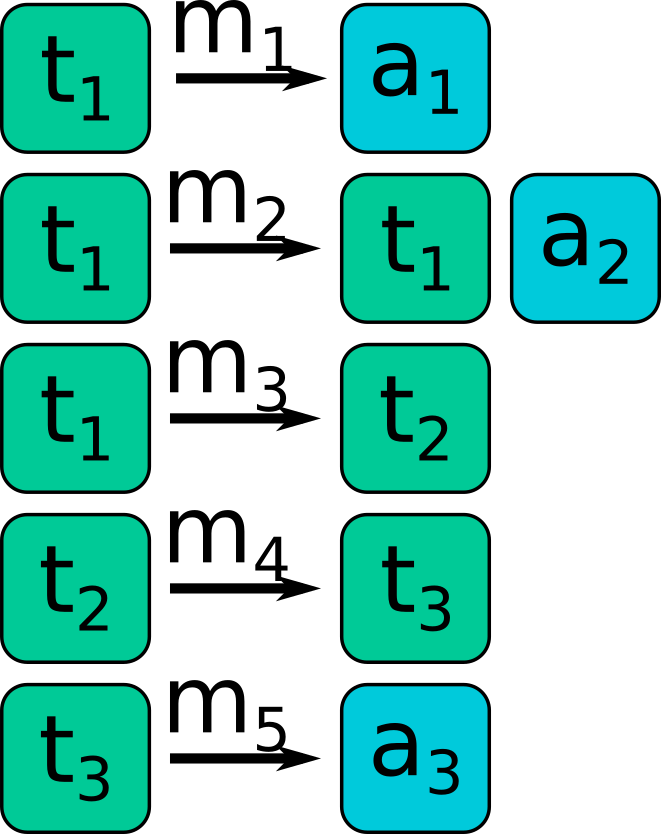
\includegraphics[width=0.3\textwidth]{images/final/heuristic_pathological_loop}
\end{figure}

\paragraph{Restarts and completeness}
Together with AMQ based loop detection, we introduced a restart mechanism in \ref{improv: loops and completeness}. We will now go over the use of restarts to achieve completeness for random DFS. \\
To show that restarts help us to achieve completeness for random DFS we can use a similar argument as we did for the loop detection. For any path in our search graph, random DFS gives us a probability $p > 0$ to take this path. As the number of restarts we perform goes to infinity, the probability to take any fixed path at least once goes to 1. We are under the same constraints as previously, needing both an unbounded number of restarts and an unbounded number of runs of at least length $u$ for any $u$. The second constraint is needed so that we do have the time to fully explore a path once we take it. Our restart mechanism fulfills both constraints, restarting with probability $\frac{1}{t}$ at second $t$. It follows that random DFS with restarts is complete.
\begin{comment}
- restarts solve the problem for DFS
- but only if we get some additional properties!
- i.e. we expect an infinite number of restarts
- additionally, we get an infinite number of runs longer than $t$ seconds for any $t$

- this is nice and gives completeness (yay!)

- loop detection also helps
- loop detection specifically helps if the wrong path is recursive
- warning: recursive does not just mean that we resolve to the same task
- two cases:
- resolve to same task, but world state is changing
- i.e., we get the exact same open tasks
- or in case of HTN we get the same open tasks and a subset of possible orderings to what we had before
- this will not immediately be detected
- however, the number of possible world states is bound
- so eventually we will find the loop, but it will take time
- resolve to the same task but also add more tasks afterwards ()
- now the open tasks are different and it is not the same search node anymore
- oh, look, an example domain
- the number of open tasks is unbounded
- heuristics cannot be saved via loop detection
- show an example domain with problems! (i.e. search nodes are not identical if we introduce additional open tasks)


- previous section \ref{improv: search completeness} talked about the completeness of different search paradigms

- Lilotane is complete (BFS-like)
- BFS search is complete
- A-star like search is complete

- we could always achieve trivial completeness, but it is not interesting from a practical perspective

- DFS and heuristic search are problematic
- DFS always has a chance to find the right path, but we have to actually hit it
- heuristic search may deterministically take the wrong way
\end{comment}

\paragraph{Conclusion}
In this section we have taken a look at completeness in hierarchical planners and how loop detection and restarts can help us to achieve it. We have shown that completeness is highly dependent on the specific search behavior with BFS-like behavior being trivially complete. In addition we show that loop detection, while helpful, is not able to solve the problem for some instances. Introducing our restart mechanism, we show that it can turn random DFS into a complete algorithm. This does not extend to heuristic DFS if the heuristic exhibits pathological behavior as the heuristic will always guide the search back into the same recursion.

\begin{comment}
- completeness is highly dependent on algorithm
- recursion remains a major challenge
- not only for runtime
- loop detection can fix many of the problems but not all
- instead of only detecting loops we may have to get better at detecting dead ends
- we may want to randomize our heuristics
- keep the benefits
\end{comment}


\section{A Malleable TOHTN Planner}
The goal of this section is to describe how we adapt it to be a malleable TOHTN planner by integrating it with Mallob, preserving both the completeness and scalability of CrowdHTN in the process. Before we get into the details, let's recall that CrowdHTN is already a moldable program according to the definition introduced in section \ref{prelim: malleability}, i.e., it may utilize any number of PEs as long as that number stays fixed during the run. We will now introduce a design that extends the parallel capabilities to achieve malleability. For this we need to address three main concerns.
\begin{itemize}
	\item Distributing the job information
	\item Integrating new PEs into a running job
	\item Dealing with PEs leaving the job while it runs
\end{itemize}
In the following sections we will address these problems in this order. Both distributing the job information and integrating new workers do not pose significant problems. Most time will be spent on the handling of disappearing PEs.
Due to the fact that we specifically integrate CrowdHTN with Mallob, in some parts we will have to refer to implementation details regarding how Mallob organizes the PEs assigned to a job as well as general message delivery.

\subsection{Distributing Jobs}
When a PE is assigned to a job, it needs to obtain a description of this job. In case of TOHTN planning, the choice is mostly between a lifted or ground TOHTN instance. Depending on pruning, a ground instance may be up to exponential in size \cite{behnke2020succinct}. Encoding and communicating such a ground instance would take up much time, which is why we decided to communicate our problem as a lifted instance. \\
With the lifted instance, we choose to simply take the textual hddl input (\cite{holler2020hddl}) and send it as-is. While this does occur the overhead of locally parsing the instance on each PE, communicating the parsed instance would involve re-encoding and effectively re-parsing it locally, too. \\
In malleable (TO)HTN planning there is a more general trade-off involved when it comes to precomputation. While parsing the instance is unavoidable, we can choose whether we want to spend time grounding and pruning our instance. It has been shown that grounding and pruning improve the planning performance (\cite{behnke2020succinct}) and allow for the computation of complex and good heuristics (\cite{holler2020htn}), but grounding, pruning and other precomputations are expensive operations themselves. As a result, a PE which is only assigned to our job for a short time may never perform any actual planning work before it is reassigned to the next job. For this reason, CrowdHTN takes an alternative path. The TOHTN instance is kept in lifted form. Instantiation is only performed as needed to explore the current search node. This allows CrowdHTN to start working immediately to utilize even short-lived PEs.
\begin{comment}
- grounded instance may be exponential in size
- exceedingly high communication cost
- lifted instance it is
- sending a parsed instance - we still need to encode and decode it for sending
- we would effectively have to build a parser for this
- we already do have a parser
- we simply encode the string and parse locally
- not a core issue to us, so we go for ease of implementation
\end{comment}

\subsection{Integrating New PEs Into Malleable CrowdHTN}
To integrate a new PE into a running TOHTN job, it needs both the general job description and part of the actual work to handle. In the previous section we explained how the job description is obtained, now we will focus on the work itself. \\
The efficient integration of new PEs into a running job is where work stealing shows it's strength. For work stealing, there is no functional difference between a PE which has locally run out of work and a new PE which has the job description but no work yet. Both will message other PEs at random to receive a new work package with no special handling required. As a result, a new PE can perform at full efficiency almost immediately, allowing our job to utilize resources as they become available.
\begin{comment}
- work stealing makes this easy
- there is functionally no difference between a new PE and a PE which has locally run out of work
- no special handling required at all

- only setup work: parsing, initiating heuristic
- CrowdHTN may be less efficient, but can work immediately, make use of very short-lived PEs
\end{comment}

\subsection{Handling PEs Leaving at Run Time}
The last challenge in designing a malleable CrowdHTN is the fact that PEs may disappear at any time. This represents a potential loss of information. The information loss presents itself in two ways. First, the loss of the local search fringe, if we do not communicate it to another PE and second, messages which may be lost in transit as their receiver no longer belongs to the same job. To deal with this, Mallob does allow us to detect locally when a PE is taken away from a job and additionally provides a message return mechanism. We will present our solutions to both cases with a focus on preserving the completeness property of CrowdHTN.

\subsubsection{Handling the Local Fringe}
When a local PE is unassigned from a job, we will loose the local search fringe. As Mallob signals a PE when it is unassigned from a job, we are however free to encode parts or all of the fringe and communicate them to another PE. This leaves us with a number of choices where we may trade-off data loss versus efficiency and communication. On this axis we discuss three choices
\begin{itemize}
	\item Encode and redistribute the whole local fringe
	\item Communicate the root of the local search space
	\item Communicate nothing, loose the local fringe
\end{itemize}

\paragraph{Encoding and redistributing the whole fringe}
Encoding and sending off the local fringe to another PE is, in a way, the easiest operation. No information is lost, preserving completeness in our planner. It does, however, come with a number of disadvantages. First, the local fringe may be arbitrarily large, especially considering that TOHTN planning is EXPSPACE-complete as seen in section \ref{prelim: tohtn complexity}. Encoding and communicating a large fringe is a very expensive operation which would increase the time from Mallob telling a PE to suspend itself until the PE actually is free for the next job. Second, receiving a large fringe would strain the memory of the receiving PE which may lead to deleting parts of it anyways to avoid crashes. Third, to avoid duplication of work as Mallob may reassign the PE to the old job, the local fringe would have to be cleared out. Doing so would weaken the effect of Mallob reassigning previously used PEs to the same job.
\begin{comment}
- the most complete operation
- nothing is lost
- nodes higher up in the tree of PEs may be more strained now (depending on the communication pattern)
- a very expensive operation
- take care to delete the local fringe to avoid duplication!
\end{comment}

\paragraph{Communicating the root of the local search space}
- easy and cheap
- duplication of work
	- re-exploring things
	- nodes that were sent off to other PEs
- how to deal with global loop detection
	- delete everything, too conservative, less performance
	- do not delete, cut off things wrongly
		- restarts deal with this increased false positive rate

- deal with disappearing workers
	- either design a scheme to preserve global knowledge or be able to deal with loss of information
	- in our case we deal with loss of information
	- two parts: loosing information stored in the fringe of a terminated node and loosing messages of dying workers
	- loosing information stored in the fringes:
		- multiple options:
			- send back nothing, loose parts of the search space
			- send back the root, redo parts of the search (also, loop detection!)
			- send back everything, takes much communication (also may duplicate the search space on resume)
			
			- our loop detection scheme already implies that we loose parts of the search space and we have measures in place to deal with this fact (restarts)
			- for this reason we go with this approach
			
\subsubsection{Handling Lost Messages}
	- loosing information due to lost messages:
		- Mallob has a mechanism to return messages
		- however, messages can still be lost (return message and original sender dies in the meantime)
		- we could change Mallob to send such messages to the root worker
		- however, this would turn the root into a bottleneck
		- again, we have mechanisms in place to deal with overall loss of information without loosing completeness
		- at the same time, we need to adapt our handling of return messages to ensure all workers stay in a valid state and do not get stuck
		- the worker may be replaced
		
	- getting wrong information (worker dies, is replaced, gets message meant for old worker)
	
	- we loose the ability to detect UNPLAN

\section{Malleable TOHTN Planning}
- upgrade from moldable to malleable task according to \cite{feitelson1997job} as introduced in section \ref{prelim: malleability}
- we can no longer assume that messages always arrive and get a response
- we want to achieve completeness
- when sending a message, we always want to send it to another 

\subsection{Adapting CrowdHTN to a Malleable Environment}
As discussed in section \ref{prelim: crowdhtn}, CrowdHTN in its original form is a moldable program, with the number of parallel workers fixed for each single execution. To adapt CrowdHTN to work as a malleable program within Mallob, we have to address three key concerns.
\begin{enumerate}
	\item Messages sent to workers who are suspended or terminated before it arrives
	\item Integrating new processes to work efficiently
	\item Dealing with workers dying without loosing completeness
\end{enumerate}
To help understanding, this section explicitly discerns between Mallob workers and Crowd workers. \todo{more terminology}
\paragraph{Messages sent to dead workers}
As Mallob runs each worker in a different processes communicating via message passing, we never have a full view of the current global state of our process, i.e., which other Mallob workers are assigned to the same job. Instead we only ever get information about this that might be outdated. As a result, when a message such as a work request is sent to another worker, we cannot be sure that the receiving worker is in a position to actually respond. Luckily, Mallob does provide us with a mechanism to detect such messages. Each Mallob worker knows which job it currently works on and all messages are tagged with their job as well. If a message belonging to job $J_i$ is received by a worker working on job $J_k, k \neq i$, the message is simply tagged with a \textit{returned to sender} flag and sent back. \\
Now we can simply adapt CrowdHTN to deal with each message both if it is received normally and if it is received as a return message. On normal messages, nothing changes. On return messages we do the following:
\begin{itemize}
	\item \textbf{Work request}: we treat this like a negative response. This means we set the \textit{has active work request} flag to false and simply send out another work request at the next chance.
	\item \textbf{Positive work response}: this is the node we sent out ourselves. As to not loose any information, we simply re-insert the node at the front of our local fringe. While this may slightly change the order of the nodes at the front, we expect the number of outgoing work packages at any point to be small and the disturbance to be limited. In case of random searches, it should not negatively affect our algorithm.
	\item \textbf{Negative work response}: we do not have to care about this and can simply ignore it.
	\item \textbf{Ack}: we do not have to care about this and can simply ignore it.
\end{itemize}
While this mechanism should deal with most cases of workers dying, we can always construct pathological cases in which the return message mechanism fails. One such exchange can be seen in graphic \ref{malleable: lost message}. One way of dealing with this would be to change the way Mallob handles messages whose receiver is no longer valid. E.g., if a return message was delivered to a worker who changed jobs in the meantime, one could instead find out the root worker of the accompanying job and send the message there instead.
\todo{ref that the root always lives at least as long as everything else}
This way no information would be lost until we decide to terminate the whole job at which point this would be unavoidable and okay by the user. To avoid having to change Mallob, we instead elected to make our adaptation of CrowdHTN resistant to such information loss.
\todo{write about loop detection and restarts here}
\begin{figure}
	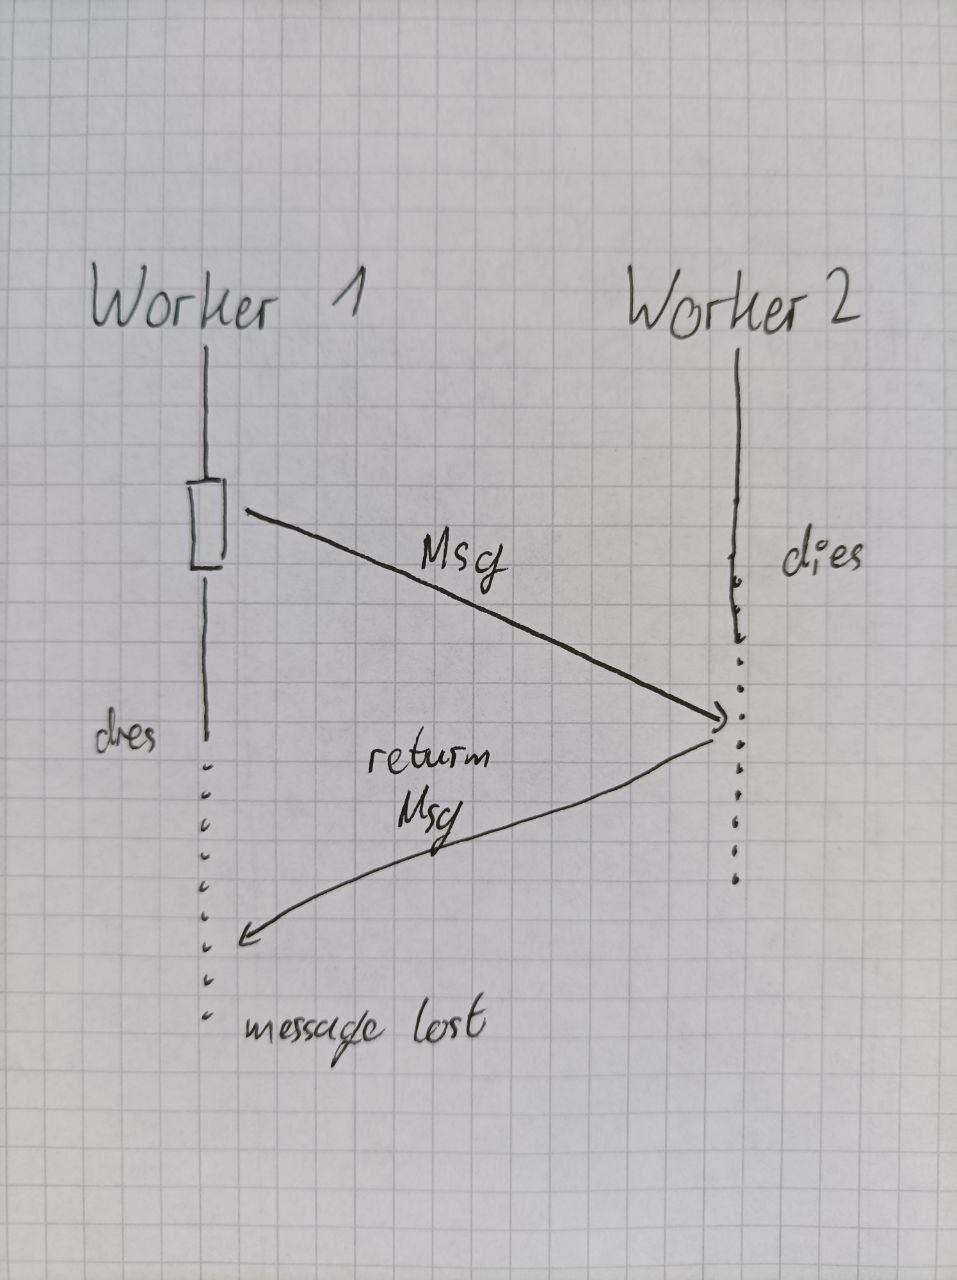
\includegraphics[width=0.6\textwidth]{images/prelim/malleable_lost_message}
	\caption{Example diagram of a lost message}
	\label{malleable: lost message}
\end{figure}

\paragraph{Integrating new workers}
As CrowdHTN uses work stealing to distribute work and perform load balancing, new workers can be seamlessly integrated into a running job. Upon construction all workers are treated the same, whether they are part of the initial batch or appear at a later point. The root worker is initialized with the initial search node, all other nodes are empty. To get new work, a worker sends a work request to a random other node and then goes from there. The very same process can be used to integrate a new worker.

\paragraph{Dealing with the information loss of dying workers}
- possible ways:
	- send back the root, delete from the loop detection -> most feasible, still looses a lot
	- send back the current fringe -> too much communication
	- ignore, do it with restarts -> easiest, we want restarts anyways. Has the consequence of loosing the UNPLAN capability as running out of work may simply be due to information loss induced by dying workers

- how to deal with workers leaving
	- hard, what if the parent is dead, too?
	- same as missing messages

- ensure completeness
- ensure performance
- work stealing is kinda nice here


\section{Implementation}
- Mallob interface (Job)
- all methods need to return fast
- have a separate worker thread
- where possible communicate via atomic bools, not locking
\subsection{Mallob Integration}
- how we integrated CrowdHTN with Mallob
- this is done by implementing a job interface in Mallob
- the interface code can be found online in the Mallob repository \footnote{https://github.com/domschrei/mallob}
- and additionally a function to read an instance
- give a short overview of the interface
- a job is internally implemented as a state machine
- the state diagram is found at \ref{figure: mallob state diagram}
- from \cite{schreiber2021scalable} we know that Mallob aims to deliver latencies in the millisecond range
- messages may only ever be sent from the main thread

\begin{algorithm}
	\caption{The Mallob job interface}
	\label{algo - mallob interface}
	void appl\_start()\;
	void appl\_suspend()\;
	void appl\_resume()\;
	void appl\_terminate()\;
	void appl\_solved()\;
	JobResult appl\_getResult()\;
	void appl\_communicate()\;
	void appl\_communicate(source, mpi\_tag, message)\;
	void appl\_memoryPanic()\;
\end{algorithm}

\subsubsection{Added Fault Tolerance}
As a scheduler, within a single execution Mallob may work on any number of jobs making it necessary that jobs do not crash. This imposes additional challenges for TOHTN planning, as we have seen in section \ref{prelim: tohtn complexity} that TOHTN planning is EXPSPACE hard, meaning we may often run out of memory and will be subsequently shut down by the operating system. Luckily, the Mallob job interface we see in algorithm \ref{algo - mallob interface} does provide a function for this case. Mallob does periodically check available memory and if it threatens to run out triggers the \textit{appl\_memoryPanic()} function. In our case we have implemented it as clearing out both our local fringe of search nodes and the loop detection information, resetting the local search. Afterwards, an affected PE will simply resume the work stealing and message other PEs to re-join the work at reduced memory footprint. While this does means we loose parts of the search space, the alternative would be to immediately return without a plan. Additionally, with the restarting mechanism we introduced in section \ref{ld - completeness} CrowdHTN retains completeness even in this case.

\subsubsection{Achieving millisecond latencies}
- big operations are put into separate threads
- this includes the \textit{start} function where the instance gets parsed and the CrowdHTN worker is initialized
- similarly, the CrowdHTN worker is put into a separate thread which is started in \textit{start}
- the functions \textit{suspend}, \textit{terminate} communicate with the CrowdHTN worker via atomics
- \textit{resume} is realized via a condition variable to wake up the worker thread
- where needed, locking is kept to an absolute minimum: messages are communicated from and to the CrowdHTN worker via dynamic arrays (realized through \textit{std::vector}) which are locked only for swapping the metadata in and out

\subsubsection{Handling version increases}
- false positives in loop detection necessitate restarts \ref{improv: loop detection}
- as a result, we need to invalidate all workers and start anew
- broadcast new versions as they happen to enforce fast updates
- loop detector size:

\begin{figure}
	\caption{State transition diagram of a Mallob job}
	\label{figure: mallob state diagram}
	\centering
	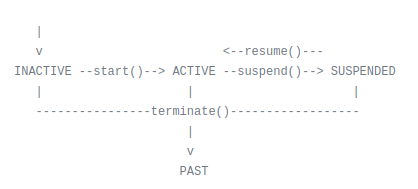
\includegraphics{images/prelim/mallob_state_diagram}
\end{figure}

\subsection{Global Loop Detection}
In section \ref{ld - global} we introduced a distributed loop detection mechanism based on regularly shared bloom filters. This leaves us with two problems, first performing the associated allreduction while the PEs assigned to the job may change at any time and secondly performing the restarts which are required if the bloom filter fills up. \\
In both cases we will make use of the specific way in which Mallob organizes the PEs assigned to a job which we have already explained in section \ref{prelim: mallob}. The two properties we rely on are the fact that PEs are internally structured as a binary tree with parent and child information available to us and the fact that the root PE will remain assigned to a job during the job's full duration.

\paragraph{Performing the Reduction}
The all-reduction of our loop detection data is initiated by the root PE and performed in three phases. 
\begin{itemize}
	\item Initiating the reduction
	\item Aggregating information upwards
	\item Broadcasting the aggregated information
\end{itemize}
The root PE is responsible for initializing the all-reduction. It does so by starting a broadcast, sending an initialization message to all it's children. Upon receiving a reduction initialization message, a PE both forwards the message to its own children and prepares the local loop detection data. 

- init: allows for a centralized start

- multiple phases:
	- 
- root induces a new sharing operation, broadcasting this information

- receiving PEs initiate their local operation, get local data, forward broadcast
- from the leaves we propagate the information upwards
- if the initiation broadcast is returned or a worker is suspended after receiving it, it's parent pretends that a message containing no data was sent
- this whole operation takes logarithmic time in the number of PEs
- if we enforce 'response exists' from bottom to top we will always conclude the operation even when PEs change

\subsubsection{Loop Detection Induced Restarts}
In section \ref{ld - global} we introduced a global loop detection mechanism based on regularly shared bloom filters. One of the problems this induces is that we need to induce restarts to increase the size of the bloom filter in order to avoid increasing false positive rates. The main problem here is that for different PEs the global bloom filter will fill up at different times. This is due to the fact that different PEs may be assigned to our job for different spans in time which may be further disjointed as PEs are suspended and subsequently reassigned to a job. However, to uphold our guarantees we want to restart all our PEs as soon as a single PE needs to do so.\\
We solve this problem by relying on the way in which Mallob organizes the PEs assigned to a single job. In section \ref{prelim: mallob} we described this organization into a binary tree of PEs. The crucial property here is that the root PE is guaranteed to stay assigned to the same job during the jobs full duration. It follows that the root PE is present during every sharing of loop detection information and that, if any PEs global bloom filter is full this implies that the root PEs global bloom filter is also full. \\
This fact allows us to only ever check on the root PE whether the global bloom filter is full and institute a restart if needed. Doing so lets us avoid any problems that would stem from all PEs performing such checks, such as multiple PEs instituting restarts at the same time.

\subsection{Improving the Search Node Exploration Algorithm}
One of the main improvements we made to the internal workings of CrowdHTN is to reduce the number of search nodes ever explicitly represented. The main idea behind this optimization is that if the next task we need to resolve is an action, then our search node has only one possible child. As such, this search node does not represent a choice point in our search and we do not need to ever explicitly instantiate it. \\
More formally speaking, let $t = t_1, \ldots, t_n$ be our sequence of open tasks. Then let $t' = t_1, \ldots, t_k$ be the longest prefix of $t$ which consists of only actions. If $k = n$, we create the next search node by applying all actions, checking preconditions and applying effects as we go. If $k < n$, we create the next search node by applying all actions in $t'$ and then additionally resolving abstract task $t_{k+1}$. \\
In addition to reducing the size of our fringe by reducing the overall number of search nodes we create, we specifically hope to save both memory and run time by reducing the number of created and represented world states. This is due to the fact that in our old algorithm resolving tasks $t_1, \ldots, t_k$ would have necessitated the creation of $k$ world states which would also not be shared as in our previously introduced scheme. Reducing the number of search nodes has additional benefits regarding loop detection. Using hash sets we reduce the memory footprint as there are fewer nodes inserted in the visited nodes set and using bloom filters the inherent probability for false positives is less of a problem the fewer nodes we check against the filter.
\begin{comment}
- first task in task network may be action
- then there is only one possible child
- the search node is not actually interesting in that it does not represent a choice point in our graph
- new definition of a search step: for sequence of open tasks $t_1, \ldots, t_k$, let $t_1, \ldots, t_m$ be the longest prefix consisting of all actions
\end{comment}
\begin{comment}
\subsection{Preceding Plan}
\todo{Section no longer valid for current crowd?}
In the initial implementation each node stored the full preceding plan as a sequence of all reductions that were applied so far. This leads to roughly quadratic overhead (sum over 1..n, only roughly as not each step increases the length. Wait, is it roughly, then? Probably, as the fraction of steps that increment the preceding plan should be kinda constant)
This duplication was not needed. The newer implementation instead stores an optional<reduction> in each node. I.e., the preceding reduction is stored if one exists, nothing if there isn't one. When the preceding plan is needed, either for communication or to extract a plan, the current search path is iterated and all reductions are accumulated.
\end{comment}

\subsection{Efficiently Hashing Nodes of the Search Graph}
As we described in section \ref{ld - perfect loop detection}, we hash a search node by hashing all of it's open tasks as well as the full world state. While the size of the world state and thus the time required to hash a world state is bound by the number of ground predicates no such limit exists regarding the open tasks. In other words, hashing both world state and open tasks has an unbounded run time which limits the effectiveness of all hash based loop detection mechanisms. In this section we will describe how we manage to reduce the time required to hash the open tasks to $\mathcal{O}(h \cdot \max \left\{ \text{\# subtasks of } r | r \in reductions \right\})$ where a single predicate can be hashed in $\mathcal{O}(h)$. \\
Let $n_1, n_2$ be search nodes with $n_2$ a child of $n_1$. Let $t_1, t_2$ be their respective sequences of open tasks with $t_1$ containing at least 1 abstract task which can be resolved by a reduction $r$ with $m$ subtasks $t_{r_1}, \ldots, t_{r_m}$. Furthermore, let $t_1 = t_{1_1}, \ldots, t_{1_k}$ with $t_{1_1}, \ldots, t_{1_l}$ the longest prefix of only actions. Then $t_2 = t_{r_1}, \ldots, t_{r_m}, t_{1_{l+2}}, \ldots, t_{1_k}$, i.e. the subtasks of $r$ concatenated with all of $t_1$ except the prefixed actions and the first abstract task. Assuming we compute our order dependent hash over a task network $t$ by going from back to front, for hashing $t_2$ we can reuse the hash of $t_{1_{l+2}}, \ldots, t_{1_k}$, only computing the hash of $t_{r_1}, \ldots, t_{r_m}$. \\
Storing the hash with each open task does increase our memory footprint. We do consider the trade-off worth it as the hash is small and it allows us to transform our hash function from an unbound to a bound run time.

\begin{comment}
- search nodes $n_1 = (t_1, s_1), n_2 = (t_2, s_2)$, $n_2$ is a child of $n_1$, assume $t_1$ contains at least 1 abstract task, resolved by reduction $r$ with $m$ subtasks
- if $t_1 = t_{1_1}, \ldots t_{1_k}$ with $t_{1_1}, \ldots, t_{1_l}$ the longest prefix consisting of only actions, then $t_2 = t_{2_1}, \ldots, t_{2_m}, t_{1_{l + 2}}, \ldots, t_{1_k}$
- i.e., $t_2$ consists of the subtasks of the applied reduction concatenated with $t_1$ except for the longest prefix of actions and one more abstract task
- our hash is order dependent, but if we hash in the order $t_{1_k}, \ldots, t_{1_1}$ we can reuse the hash of $t_{1_k}, \ldots, t_{1_{l+2}}$ for $n_2$, only computing new hashes for $t_{2_m}, \ldots, t_{2_1}$
- this is possible in $\mathcal{O}(h \cdot m)$ where a single predicate can be hashed in time $\mathcal{O}(h)$

Overview:
\begin{itemize}
\item the hash of a node consists of two parts
\item 1: the hash of the open tasks
\item 2: the hash of the world state
\item We do not care about the hash of the preceding plan. Nodes with open tasks and world state equivalent have equivalent plans leading to a goal (somewhat similar to the Nerode relation) and we do not care about optimality. How he reach this point with equivalent remaining options is thus not of interest to us
\item The hash of the world state can be large, but the number of elements is ultimately bound for any particular instance
\item The length of the preceding plan is unbounded
\end{itemize}
Open tasks:
\begin{itemize}
\item Care needs to be taken to use an order independent hash function for the world state, as the underlying representation as a set does not guarantee us any particular iteration order, especially between nodes (might depend on the order of things inserted into the set!)
\item Alternatively we could have chosen some other ordered representation, e.g. maintain the world state as a sorted list of predicates with a defined order. This would imply extra work we are unwilling to do.
\item For open tasks, we save not only the task itself but additionally the hash of all open tasks from first to current one
\item The order in which we hash open tasks is from oldest to newest one
\item On applying a Reduction, we push the new open tasks onto the open task stack and compute each of their hashes combined with their predecessors. Each of these hashing operations is completed in O(1)
\item Effectively, this means that each task is hashed exactly once
\item As we already have to push each task onto the open tasks, inserting an additional O(1) operation on pushing does not change the asymptotic runtime
\end{itemize}

The same technique is used to efficiently compute our heuristic presented in section \ref{improv: crowd heuristic}

World state:
\todo{this is not implemented yet, take care to actually bring it into Crowd}
\begin{itemize}
\item In section XXX \todo{add section, refer to it here} we discussed how each copy of the world state can be shared by many search nodes to reduce the memory footprint
\item Instead of hashing the world state each time on demand, we can store a shared tuple of world state and it's hash
\item This way, we only hash the world state once, reusing the computation
\item Is this actually a time saving?
\todo{Only put node into loop detection as it is explored, so we can always keep exploring the local node (the node we are colliding with may be arbitrarily far back in our fringe)}
\todo{Evaluate how many world state hashes we actually compute in both cases. Hashing a world state of a node which is ultimately not explored (and which is otherwise not needed) is wasted.
Number of computations on lazy hashing: number of nodes created - number of nodes remaining in fringe on plan found}
\item Future work: the hash of the world state is order independent (sum of squares of individual hashes), to not worry about forcing any fixed iteration order. Utilize this and wrapping maths to hash only the differential of 
\end{itemize}
\end{comment}

\begin{comment}
\subsection{Lazy Instantiation of Child Nodes}
lazy instantiation works on the basis of finding all free variables of a method and creating Reductions based on all possible combinations

Initial implementation: instantiate all possible reductions, filter out any with not fulfilled preconditions,then shuffle them

Problems: this spends both time and memory instantiating reductions that might never be needed for the rest of the search
We effectively save not only the current path, but also follow all possible branches to a distance of 1

Solution: lazily create reductions as needed
How to do this (first way):
adapt the argiterator from Lilotane into the CrowdHTN code base. Adapt it to only substitute the arguments that are not already determined by the corresponding task (arguments)

To achieve randomization:
each domain is iterated to create the substitutions
Each time we build such an iterator, we randomize the order within the domains for this specific iterator
This will lead to different orders

Further ideas:
each time domains 1..k have been fully iterated, increment k+1 by 1, then shuffle the order of domains 1..k

For n total domains, each time domains 1..n-1 have been iterated, remove the current value from domain n, then shuffle all domain orders

Compare the runtimes of eager and lazy instantiation, check at which point it is worth it to incur the (potential) additional overhead of lazy instantiation
Compare on multiple domains?
Check different metrics for comparison (size of domains, number of parameters, number of potential children (product of sizes))

Potential problems:
We need quite a bit of state (domains, current index into each domain) to perform lazy instantiation
The order is not truly random. We iterate some domains faster/ more often than others. What if the important change is in a domain which is iterated slowly? More random order makes this easier

A potential solution: space filling curves
Advantages: little state (can just be incremented), iterates all dimensions equally
Disadvantage: fixed order. With shuffling within each domain might be random again

Space filling curves come with the restriction of being strictly continuous
We do not need this property. All we are interested in is an easy to compute fixed order in which the whole space is iterated where each permutation is hit exactly once
We want only self-avoiding curves, to not hit any instantiation twice (could loop detection just fix that? But it would be a bad fix)
\end{comment}


\section{Experimental Evaluation}

\subsection{Experimental Setup}
\label{eval: setup}
In our evaluation we reuse the reduced IPC benchmark set we introduced in \cite{bretl2021parallel}.
We use them, as they remain the de-facto standard for evaluating hierarchical planners \cite{schreiber2021lilotane, holler2020htn, holler2021landmark, bretl2021parallel}.
The selection consists of 120 out of the 892 instances used in the IPC 2020, using 5 instances per domain and using 900 seconds per run instead of the 30 minutes in the IPC to make evaluation of many different planner configurations more feasible. \\
We define the run time of a planner as follows:
\begin{itemize}
	\item From start until a plan is printed for standalone planners. This includes time spent parsing and grounding
	\item The wallclock time measured by Mallob for our malleable CrowdHTN, again including parsing
\end{itemize}
Planners are scored according to both the IPC score and coverage. The IPC score is defined as 1, if a plan was found in less than 1 second, 0 if no plan was found and for $0 < t < 900$ as
\[
1 - \frac{log(t)}{log(T)}
\]
Our tests were done on two machines. The first is a server with an Intel Xeon Gold 6138 processor with 4 sockets, 20 cores per socket and 2 threads per core clocked 2.00G Hz with around 750GB of RAM and running Ubuntu 20.04. We will call it PC1. The second is a server with an AMD EPYC 7702 processor with 1 socket with 64 cores and 2 threads per core clocked 2.00 GHz with around 1TB of RAM and running Ubuntu 20.04. We will call it PC2. \\
As for sequential planners, we offer a short comparison with PANDA and HyperTensioN specifically, as those are also search-based planners with overall similar characteristics. 

\paragraph{Naming Scheme}
As our CrowdHTN planner contains multiple configuration options, we use a succinct naming scheme to identify them in the evaluation. The name for a CrowdHTN configuration has the following structure:
\[
	\text{Cr}
	\left\langle \text{CrowdHTN version} \right\rangle
	\left\langle \# \text{of PEs} \right\rangle
	\left\langle \text{loop detection method} \right\rangle
	\left\langle \text{presence of restarts} \right\rangle
\]
A list of possible values for each category as well as their meaning is shown in table \ref{table: crowd configs}. The use of a global bloom filter always implies the use of probabilistic restarts. Unless noted otherwise, all configurations of CrowdHTN use randomized DFS.
\begin{table}[!hbp]
	\caption{List of parameters identifying a CrowdHTN configuration}
	\label{table: crowd configs}
	\centering
	\begin{tabular}{|l|l|l|}
		\hline
		Parameter & Value & Meaning \\
		\hline
		CrowdHTN Version & O & Old CrowdHTN, standalone \\
		 			     & N & New CrowdHTN, integrated with Mallob \\
		\hline
		Loop Detection Method & Hs & Hash Set \\
							  & Bl & Local Bloom Filter \\
							  & Bg & Global Bloom Filter \\
							  & No & No loop detection \\
		\hline
		Presence of Restarts & R & Time dependent restarts are used \\
							 & / & No time dependent restarts are used \\
		\hline
	\end{tabular}
\end{table}

\begin{comment}
CrowdHTN metadata
- same instance set
- 300 seconds per instance
- log the run time behavior regarding the search behavior
- 64 cores, 2 GHz max
- AMD EPYC 7702
- around 1 TB of RAM
- Ubuntu 20.04
\end{comment}

\subsection{Comparing to old CrowdHTN}
\label{eval: old}
When comparing our new implementation of CrowdHTN with the old CrowdHTN, we do see an overall higher IPC score while retaining coverage for our best version where all new features are active. However, when comparing old CrowdHTN with the new implementation using hash sets for loop detection, we note a loss in both coverage and IPC score. A plot of their respective performances is shown in figure \ref{figure: eval old new}. \\
We suspect that the performance degradation comes from our integration into Mallob. CrowdHTN as a work stealing planner sends a high number of messages. As we have seen in the implementation section, to uphold the guarantees of Mallob we do not directly communicate and instead write messages into separate buffers for Mallob to receive and send on which we suspect as one area of lost performance. Additional small overhead may be due to the fact that Mallob performs additional scheduling and rebalancing work in the background, though we expect these effects to be rather small.\\
However, the improvements we added to CrowdHTN do make up for these losses. Additionally, our new implementation of CrowdHTN generally achieves a higher IPC score per coverage, i.e., if a plan is found it was found fast. If this only happened in badly performing configurations, we would suspect that only easy problems with a high score are solved anymore. However, this correlation holds for all configurations of new CrowdHTN, even those exceeding the old version.
\begin{figure}
	\caption{Plotting instances solved per time for old and new CrowdHTN}
	\label{figure: eval old new}
	\centering
	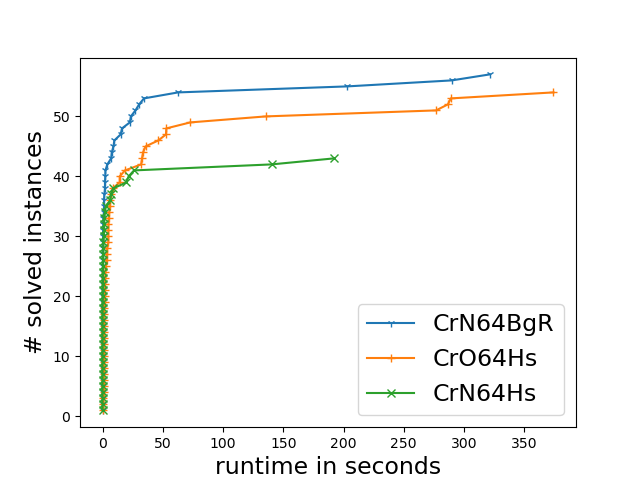
\includegraphics[width=0.5\textwidth]{images/final/old_new}
\end{figure}
Compared to sequential planners PANDA and HyperTensioN, results are mixed.
Looking at PANDA, compared to old CrowdHTN we manage to catch up in domains Hiking Monroe-Fully-Observable and Snake while staying ahead on Blocksworld-HPDDL, Minecraft-Player and Rover-GTOHP. However, overall CrowdHTN still looses out to the more informed PANDA planner. \\
When looking at HyperTensioN, CrowdHTN retains the advantage of high coverage as it's distributed nature makes it less hit-or-miss than HyperTensioN itself. At the same time, improvements in time to plan mean that CrowdHTN almost catches up to HyperTensioN regarding IPC score.

\subsection{Optimizations in CrowdHTN}
\label{eval: crowd optimizations}
In \ref{impl: reduce nodes} we described an improvement to our progression search which let us reduce the number of search nodes we instantiate. To evaluate the impact of this improvement we created an instrumented version of CrowdHTN which let us track this information during planning. We ran this version of CrowdHTN on our benchmark on PC2, using 1 PE, DFS and hash set based loop detection while giving it 300 seconds per instance. We tracked the metadata for all instances, whether a plan was found or not. In addition to the information on actions and world states, we tracked the number of search nodes which were duplicates. The results are shown in table \ref{table: tohtn metadata}. \\
Compared to the other measures, the ratio of tasks which are actions is relatively consistent between domains. It varies from about one third to about two thirds of all tasks. The ratio is lowest for the Logistics-Learned-ECAI-16 domain at $28.2\%$ and highest for Rover-GTOHP at $66.83\%$. \\
When it comes to shared world states, results vary more. On 11 out of the 24 test domains, a world state is on average shared by less than 10 search nodes. This is lowest for the Snake domain with only $1.4$ search nodes per world state. On the other hand for 6 out of our 24 domains more than $1000$ search nodes share one world state, going as far as $\sim3.5 \times 10^8$ search nodes per world state for the Transport domain. \\
To sum these improvements up, our improved search node exploration is a clear benefit on all domains, reducing the number of search nodes we need to represent by at least $28\%$. Sharing world states is more mixed. While sharing is extreme on some domains, it does come at the cost of an additional pointer indirection which may be harmful on domains with little sharing. \\
Regarding loop detection, the results are similarly varied as with state sharing. On 7 out of 24 domains no duplicate nodes were encountered at all and on another 5 domains less than 1\% of nodes were duplicates. At the other end of the spectrum we have Minecraft-Player and Logistics-Learned-ECAI-16 with $\sim30\%$ and Factories-simple with $\sim44\%$ of duplicate nodes. We will return to these numbers in the evaluation of different loop detection techniques in \ref{eval: loop detection}.
\begin{table}[!hbp]
	\caption{Metadata about progression search on our benchmark}
	\label{table: tohtn metadata}
	\centering
	\begin{tabular}{|l|c|r|r|}
		\hline
		Domain & Action\% & Nodes per World State & Loop\% \\
		\hline
		AssemblyHierarchical & 49.71 & 4793.8 & 0.006\\
		Barman-BDI & 33.56 & 10.4 & 4.866\\
		Blocksworld-GTOHP & 50.80 & 6.1 & 0.000\\
		Blocksworld-HPDDL & 49.34 & 83.4 & 1.690\\
		Childsnack & 53.94 & 28800.6 & 0.000\\
		Depots & 45.11 & 7.3 & 2.790\\
		Elevator-Learned-ECAI-16 & 47.89 & 44.9 & 1.663\\
		Entertainment & 49.49 & 7.2 & 0.095\\
		Factories-simple & 31.09 & 2.3 & 43.815\\
		Freecell-Learned-ECAI-16 & 44.42 & 2.5 & 0.000\\
		Hiking & 65.24 & 2.6 & 12.508\\
		Logistics-Learned-ECAI-16 & 28.20 & 4.7 & 30.348\\
		Minecraft-Player & 32.21 & 4.4 & 29.896\\
		Minecraft-Regular & 31.34 & 3.4 & 0.000\\
		Monroe-Fully-Observable & 48.65 & 114.0 & 1.457\\
		Monroe-Partially-Observable & 48.29 & 106.6 & 3.418\\
		Multiarm-Blocksworld & 47.06 & 28.9 & 8.240\\
		Robot & 50.00 & 46207.3 & 0.002\\
		Rover-GTOHP & 66.83 & 3.5 & 0.000\\
		Satellite-GTOHP & 34.66 & 52.5 & 0.013\\
		Snake & 47.16 & 1.4 & 6.948\\
		Towers & 49.99 & 5409.3 & 0.000\\
		Transport & 36.98 & 347788104.5 & 0.000\\
		Woodworking & 49.83 & 21708.8 & 0.442\\
		\hline
	\end{tabular}
\end{table}

\subsection{Search Algorithms}
\label{eval: algorithms}
In section \ref{improv: search algorithms} we presented four search algorithms that we implemented for CrowdHTN. Those algorithms are random DFS, heuristic DFS, A-star like and BFS. We have tested all four algorithms on our test instance set using 4 PEs and a local bloom filter without restarts for loop detection. The results of this test are visualized in figure \ref{figure: eval algorithm}, a summary of coverage and IPC score is presented in table \ref{table: eval algorithm}. \\
Overall, random DFS performed best, followed by heuristic DFS, A-star like search and finally BFS with our best algorithm, random DFS, solving almost twice as many instances and having twice the IPC score of our worst algorithm, BFS. Additionally, we observe a hit-or-miss behavior in both our DFS implementations where plans are either found almost immediately or not at all. Out of the 50 instances solved by random DFS, only 18 were solved in more than 1 and out of these 18 only 9 were solved in more than 10 seconds. BFS on the other hand solves 14 out of 30 instances in more than a second and 11 of these 14 in over 10 seconds. As such, while overall worse performing it does seem to scale better with runtime. Overall, BFS seems unsuited for TOHTN planning due to the extremely high branching factor of the problems involved.
\\
Comparing our two DFS-based approaches, we see that random DFS performs better than heuristic DFS guided by our heuristic from section \ref{improv: crowd heuristic}. We attribute this to the fact that we consciously limited our heuristic to information on the hierarchy available from the lifted instance to reduce the time spent on precomputation. Others, such as \cite{holler2020htn} argue that heuristics must utilize both hierarchy and world state information. Our findings corroborate this theory.

\begin{figure}[!hbp]
	\caption{Plotting the number of solved instances per run time for CrowdHTN using DFS, heuristic DFS, A-star like search and BFS}
	\label{figure: eval algorithm}
	\centering
	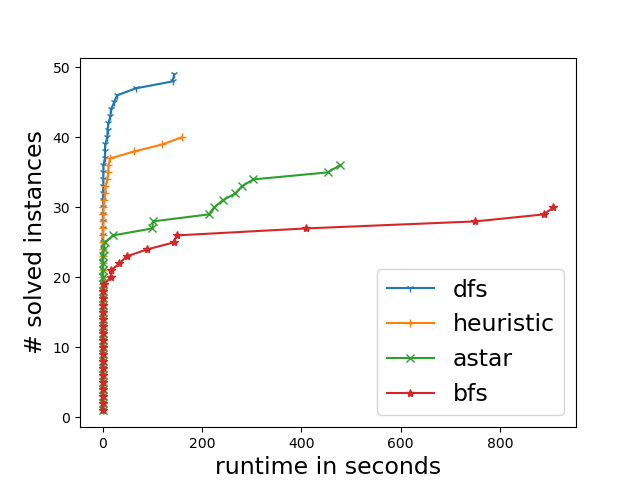
\includegraphics[width=0.5\textwidth]{images/final/search_algorithms.png}
\end{figure}
\begin{table}[!hbp]
	\caption{Coverage and IPC score of our search algorithms using 4 PEs and a local bloom filter}
	\label{table: eval algorithm}
	\centering
	\begin{tabular}{| l | r | r |}
		\hline
		Algorithm 		& Coverage & IPC Score \\
		\hline
		Random DFS 		& 41.7\%	& 43.09 \\ % 50
		Heuristic DFS 	& 33.3\%	& 35.60	\\ % 40
		A-star like 	& 38.3\%	& 27.13 \\ % 36
		BFS 			& 25.0\%	& 21.87	\\ % 30
		\hline
	\end{tabular}
\end{table}

\subsection{Bloom Filters in Loop Detection}
\label{eval: loop detection}
The next feature we tested was the new loop detection based on bloom filters. For our tests we set $k=4$ and limited our false positive probability to $0.001$. The results of this test are shown in figure \ref{figure: eval loop detection}. We see that our bloom filter outperforms the hash set on 32 and 64 PEs, increasing the IPC score by $\sim 5.5$ and coverage by about 6\% when switching from hash set to bloom filter. The gains are so large that 32 PEs using a bloom filter outperform 64 PEs using a hash set. \\
The gains are strongest on the domain Monroe-Fully-Observable and also visible on Snake.
However, we also note that our hash set based loop detection achieves good performance on the Logistics-Learned-ECAI-16 domain while no configuration using bloom filters was able to solve a single instance on this domain. A similar but weaker effect happens in Factories-simple.
Looking at the data in table \ref{table: tohtn metadata} we see that Logistics-Learned-ECAI-16 and Factories-simple are two of the domains with the highest rate of duplicate nodes. We are not sure why Minecraft-Player, the last domain with very high prevalence of duplicate nodes, does not exhibit the same behavior.

\begin{figure}[!hbp]
	\caption{Evaluating CrowdHTN with hash set and bloom filter based loop detection}
	\label{figure: eval loop detection}
	
		\centering
		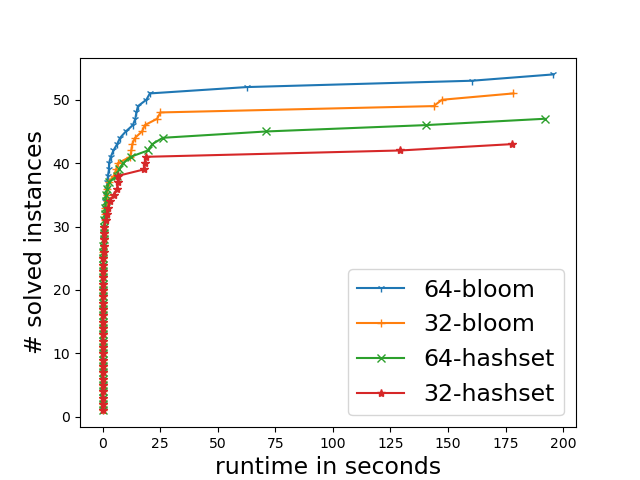
\includegraphics[width=0.5\textwidth]{images/final/loop_detection}
\end{figure}

\subsection{Probabilistic Restarts and Global Loop Detection}
\label{eval: restarts}
In our next test, we enabled the probabilistic restarts we introduced to guarantee completeness for our bloom filter based loop detection. With runs lasting 900 seconds, we expect $\sum_{t=1}^{899} \frac{1}{t} \approx 7.38$ restarts per run with 5 of these restarts happening within the first 90 seconds. \\
First, we compare CrowdHTN using local bloom filters with and without restarts. The result is shown in figure \ref{figure: restarts}. Overall, probabilistic restarts seem to have a positive effect on coverage and IPC score which is more pronounced on a lower number of PEs. In this way they somewhat mitigate the hit-or-miss nature of our planner. \\
While we see a big difference on 32 PEs, there is little difference on 64 PEs where restarts come with a slight benefit to coverage and a little loss in IPC score. We suspect that, while restarts may increase our chances of finding a plan, they do decrease the chance of finding a plan fast, as they interrupt our search and are especially common right at the beginning. Additionally, there is little difference between restarts on 32 and 64 PEs. We will go further into the specific scaling behavior of CrowdHTN in the benchmark on scalability in \ref{eval: scalability}. \\
\begin{figure}[!hbp]
	\caption{Evaluating CrowdHTN with a local bloom filter with and without restarts}
	\label{figure: restarts}
	\centering
	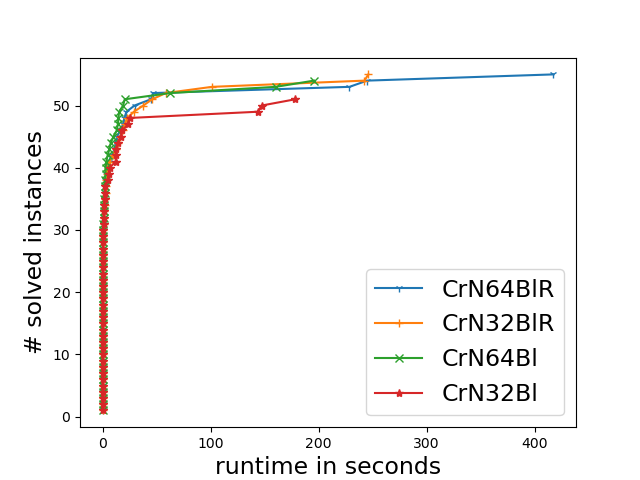
\includegraphics[width=0.5\textwidth]{images/final/restarts}
\end{figure}

\subsection{Global Loop Detection}
\label{eval: global loop}
The last new feature we introduced into CrowdHTN is the ability to perform distributed loop detection and plotted the results in figure \ref{figure: global loops}. Comparing it to CrowdHTN with restarts but no shared information about known search nodes, we get a further small increase in both coverage and IPC score. Among all configurations using bloom filters, CrowdHTN on 64PEs and using global loop detection has the highest coverage and the overall highest IPC score. Similarly, the configuration on 32 PEs is the second best overall, slightly outperforming the 64 PE versions with and without restarts.

\begin{figure}[!hbp]
	\caption{Comparing CrowdHTN with a local bloom filter and restarts with global loop detection}
	\label{figure: global loops}
	\centering
	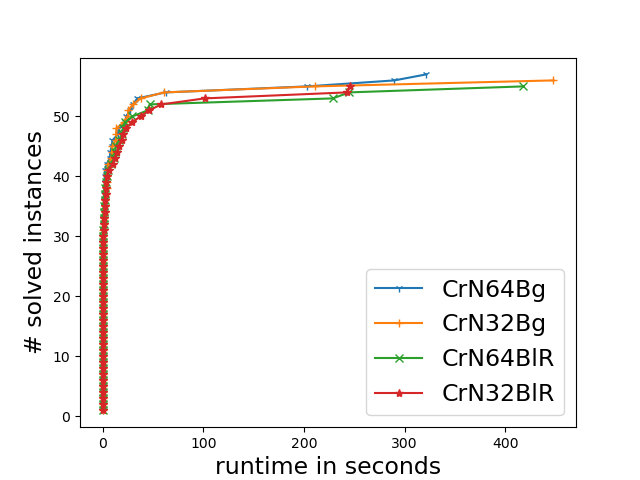
\includegraphics[width=0.5\textwidth]{images/final/global_loops}
\end{figure}

\subsection{Scalability of CrowdHTN}
\label{eval: scalability}
As CrowdHTN is a search-based planner, it has a hit-or-miss characteristic to its performance. This can make it hard to see how its overall performance scales. Many instances are already efficiently solved on a low number of PEs while other instances will remain out of reach even on a high number of PEs. However, over our full benchmark we can still see an increase in overall performance as seen in figure \ref{figure: eval scalability}, even if the effect is relatively weak. \\
To better visualize the scaling behavior of CrowdHTN we will now focus on the Monroe-Fully-Observable domain. It has instances which are somewhat reliably solved for any number of PEs while not being trivial. We ran a separate benchmark of all 20 instances that come with this domain on PC2, testing various configurations of CrowdHTN with local loop detection and no restarts versus global loop detection with restarts. The results are listed in table \ref{table: eval scalability}.\\
Overall we note the clearly increasing IPC score as the number of PEs is increased. Increasing the number of PEs from 4 to 16 has a bigger effect than quadrupling it again to 64. We assume that on this test benchmark the chance of encountering a plan is sufficiently high that we run into diminishing returns as the number of PEs is increased further. Interestingly, CrowdHTN without restarts seems to scale more strongly than CrowdHTN with restarts, as far as the IPC score is concerned. We attribute this to the fact that the IPC score values short run times especially high. Restarts are most frequent during the early phase of planning and may stop CrowdHTN from finding plans very fast. \\
To reduce the impact of randomness, we launched on additional test using instance 11 of the Monroe-Fully-Observable domain. We used CrowdHTN with global loop detection and restarts active, running it 100 times with a time limit of 90 seconds. The distribution of run times is shown in figure \ref{figure: eval scalability box} while success rate and average run times are listed in table \ref{table: eval scalability 2}. All three configurations have high success rate, at 93\%, 97\% and 98\% respectively. The addition of 8 more PEs correlates with an approximately 10 second decrease in average run time. This corresponds to a percentage decrease in run times of 20\% when going from 16 to 24 PEs and of another 30\% when going from 24 to 32 PEs, increases in PEs of 50\% and 33\% respectively.
In reality, gains are even higher as these average run times ignore the cases were the 16 PE configuration failed to find a plan at all.

\begin{figure}[!hbp]
	\caption{Plotting the number of solved instances per run time for CrowdHTN using DFS and a local bloom filter on 64, 16 and 4 PEs}
	\label{figure: eval scalability}
	\centering
	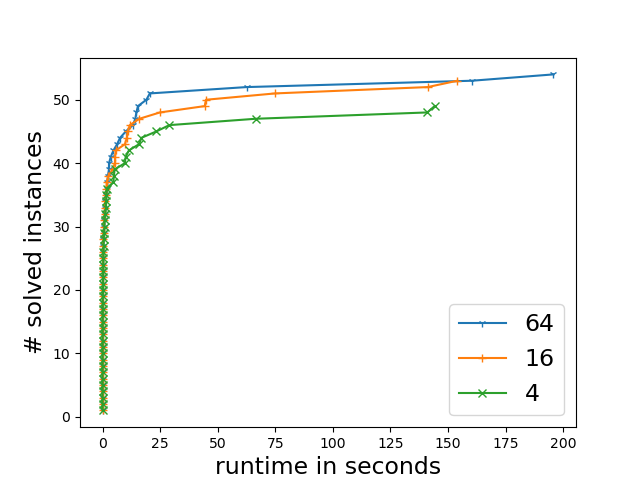
\includegraphics[width=0.5\textwidth]{images/final/scalability}
	% python3 ../MA_scripts/diagrams.py -files=results_64_dfs_local_bloom.csv,results_16_dfs_local_bloom.csv,results_4_dfs_local_bloom.csv  -names=64,16,4
\end{figure}
\begin{table}[!hbp]
	\caption{Evalutating CrowdHTN on 20 instances of the Monroe-Fully-Observable domain}
	\label{table: eval scalability}
	\centering
	\begin{tabular}{|l|rc|rc|rc|rc|rc|rc|}
		\hline
		& \multicolumn{2}{c|}{\textbf{CrN4Bl}} & \multicolumn{2}{c|}{\textbf{CrN16Bl}} & \multicolumn{2}{c|}{\textbf{CrN64Bl}} & \multicolumn{2}{c|}{\textbf{CrN4Bg}} & \multicolumn{2}{c|}{\textbf{CrN16Bg}} & \multicolumn{2}{c|}{\textbf{CrN64Bg}}\\
		& Time & IPC & Time & IPC & Time & IPC & Time & IPC & Time & IPC & Time & IPC\\
		\hline
		01 & 0.2 & 1.00 & 0.1 & 1.00 & 0.4 & 1.00 & 0.1 & 1.00 & 0.7 & 1.00 & 0.1 & 1.00\\
		02 & 161.5 & 0.25 & 30.7 & 0.50 & 1.3 & 0.96 & 115.6 & 0.30 & 10.5 & 0.65 & 22.6 & 0.54\\
		03 & / & 0.00 & 5.7 & 0.74 & 8.4 & 0.69 & 250.5 & 0.19 & 4.0 & 0.80 & 30.5 & 0.50\\
		04 & 0.4 & 1.00 & 0.3 & 1.00 & 0.2 & 1.00 & 0.3 & 1.00 & 0.3 & 1.00 & 0.4 & 1.00\\
		05 & 49.9 & 0.43 & 55.6 & 0.41 & 22.6 & 0.54 & 23.7 & 0.53 & 30.2 & 0.50 & 26.6 & 0.52\\
		06 & 183.9 & 0.23 & 60.1 & 0.40 & 3.5 & 0.82 & 129.0 & 0.29 & 61.7 & 0.39 & 18.2 & 0.57\\
		07 & 18.5 & 0.57 & 7.2 & 0.71 & 3.2 & 0.83 & 5.3 & 0.75 & 2.0 & 0.90 & 4.0 & 0.80\\
		08 & 98.1 & 0.33 & 48.0 & 0.43 & 4.4 & 0.78 & 108.0 & 0.31 & 101.7 & 0.32 & 12.5 & 0.63\\
		09 & 62.3 & 0.39 & 17.7 & 0.58 & 26.0 & 0.52 & 70.8 & 0.37 & 13.5 & 0.62 & 14.3 & 0.61\\
		10 & 122.1 & 0.29 & 33.9 & 0.48 & 23.8 & 0.53 & 80.4 & 0.35 & 61.9 & 0.39 & 11.0 & 0.65\\
		11 & 148.9 & 0.26 & 60.5 & 0.40 & 15.7 & 0.60 & 148.6 & 0.26 & 62.8 & 0.39 & 15.0 & 0.60\\
		12 & 137.5 & 0.28 & 47.9 & 0.43 & 19.4 & 0.56 & 223.4 & 0.20 & 34.7 & 0.48 & 25.6 & 0.52\\
		13 & 19.4 & 0.56 & 2.7 & 0.85 & 1.5 & 0.94 & 7.9 & 0.70 & 0.6 & 1.00 & 1.7 & 0.92\\
		14 & 171.3 & 0.24 & 61.1 & 0.40 & 36.1 & 0.47 & 279.5 & 0.17 & 36.2 & 0.47 & 42.1 & 0.45\\
		15 & / & 0.00 & 6.5 & 0.73 & 4.3 & 0.79 & / & 0.00 & 5.0 & 0.76 & 0.8 & 1.00\\
		16 & / & 0.00 & 6.3 & 0.73 & 2.0 & 0.90 & 7.1 & 0.71 & 6.2 & 0.73 & 4.8 & 0.77\\
		17 & / & 0.00 & 1.6 & 0.93 & 11.2 & 0.64 & / & 0.00 & / & 0.00 & 1.8 & 0.91\\
		18 & 16.7 & 0.59 & 40.0 & 0.46 & 10.3 & 0.66 & 47.2 & 0.43 & 9.0 & 0.68 & 37.7 & 0.47\\
		19 & 1.9 & 0.90 & 5.1 & 0.76 & 1.8 & 0.91 & 15.7 & 0.60 & 15.0 & 0.60 & 5.7 & 0.74\\
		20 & 21.7 & 0.55 & 2.9 & 0.84 & 2.5 & 0.86 & 12.5 & 0.63 & 6.0 & 0.74 & 4.6 & 0.78\\
		\hline
		& & 7.88 & & 12.78 & & 15.01 & & 8.81 & & 12.43 & & 13.98\\
		\hline
	\end{tabular}
\end{table}
\begin{figure}[!hbp]
	\caption{Distribution of run times on Monroe-Fully-Observable instance 11}
	\label{figure: eval scalability box}
	\centering
	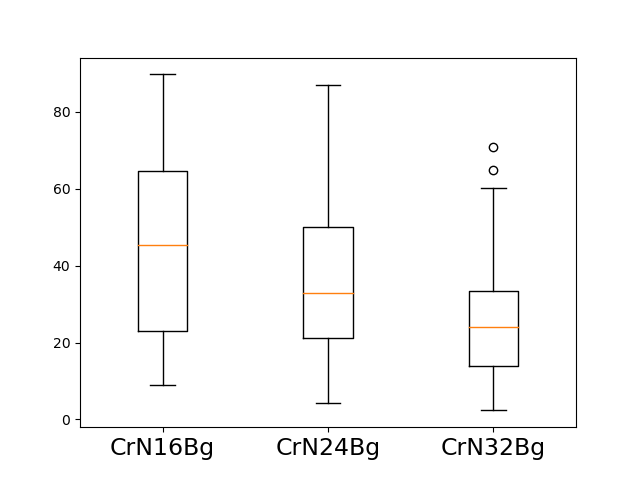
\includegraphics[width=0.5\textwidth]{images/final/scalability_2}
\end{figure}
\begin{table}[!hbp]
	\caption{Success rate and average, minimum and maximum run times of CrowdHTN on Monroe-Fully-Observable instance 11}
	\label{table: eval scalability 2}
	\centering
	\begin{tabular}{|l|c|c|}
		\hline
		Configuration & Success Rate & Average time to plan \\
		\hline
		CrN16Bg 	& 93\% & 45.73  \\
		CrN24Bg		& 97\% & 36.62  \\
		CrN32Bg		& 98\% & 25.98  \\
		\hline
	\end{tabular}
\end{table}

\subsection{Malleable CrowdHTN}
\label{eval: malleable}
To test the behavior of CrowdHTN under malleable conditions, we extended our previous test on scalability. We ran another test on Monroe-Fully-Observable instance 11 using 32 PEs. However, every 20 seconds we injected a second unsolvable job with a time limit of 10 seconds. This means that our normal test oscillates between 32 and 16 PEs every 10 seconds, having an average of 24 PEs available. We compare success rate, average time to plan and the overall distribution of run times with moldable CrowdHTN on 24 PEs. The results are listed in table \ref{table: malleability}. Figure \ref{figure: malleability} shows a box plot of run times per solver. \\
Moldable CrowdHTN on 24 PEs reliably solves this problem in 90 seconds with a success rate of 97\% and an average time to plan of 36.62 seconds. In the ideal case, our malleable CrowdHTN would replicate this behavior. However, we see that malleable CrowdHTN achieves only 69\% success rate with an average time to plan of 31.84 seconds. Looking at the box plot visualizing the distribution of run times, we see that malleable CrowdHTN and moldable CrowdHTN on 24 PEs share the distribution of run times of up to about 50 seconds. Malleable CrowdHTN is missing tail end of the distribution, though, finding no plans beyond the 60 second mark. \\
We suspect that this behavior is due to the way restarts are implemented in CrowdHTN and with how disappearing workers are handled. As we restart with probability $\frac{1}{t}$ at second $t$, we expect about 5 restarts during a 90 second run with 4 of these restarts taking place in the first 30 seconds. Additionally, we handle disappearing PEs by sending the root of their local search space to a random other PE. As in our experiment half of PEs are lost each time another job is introduced, a high number of those messages may be sent to other disappearing PEs, leading to an unexpectedly high loss of information. Restarts seem to mitigate this at the beginning of the search as they are still frequent.
\begin{figure}[!hbp]
	\caption{Distribution of solving times for malleable and moldable CrowdHTN}
	\label{figure: malleability}
	\centering
	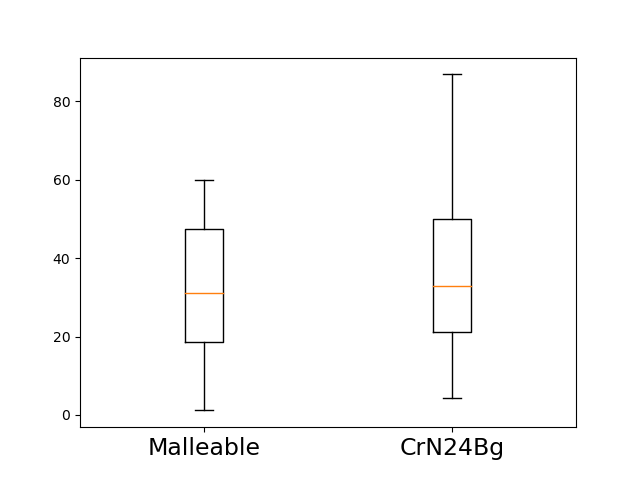
\includegraphics[width=0.5\textwidth]{images/final/malleability}
\end{figure}
\begin{table}[!hbp]
	\caption{Coverage and average run time of malleable and moldable CrowdHTN}
	\label{table: malleability}
	\centering
	
	\begin{tabular}{|l|c|c|}
		\hline
		Configuration & Success rate & Average time to plan \\
		\hline
		Malleable, average 24 PEs	& 69\%	& 31.84 \\
		CrN24Bg						& 97\%  & 36.62 \\
		\hline
	\end{tabular}
\end{table}

\subsection{Discussion}
\label{eval: conclusion}
In this section, we compare our parallel TOHTN planner CrowdHTN as it is integrated into Mallob to the old standalone version of CrowdHTN as well as sequential planners PANDA and HyperTensioN. As shown in the previous sections, the integration of CrowdHTN into Mallob comes with some amount of overhead. We show that CrowdHTN has it's own specific strengths and manages to outperform HyperTensioN in coverage while coming close in overall score. \\
We see the following main results
\begin{itemize}
	\item Our improved node exploration algorithm manages to reduce the number of instantiated nodes from around one to two thirds total.
	\item Bloom filters in loop detection improve both coverage and IPC score overall with the bigger impact on IPC score.
	\item Distributed loop detection and restarts improve coverage and IPC score for smaller numbers of PEs while increasing coverage but potentially decreasing IPC score for a large number of PEs. This may be due to the fact that very fast times to plan are lost in early restarts.
\end{itemize}
Regarding our upgrades to CrowdHTN, we see that the improved node exploration algorithm leads to a big reduction in overall search nodes encountered. Furthermore, bloom filters and distributed loop detection along with restarts both manage to improve the performance of CrowdHTN, with the bigger gain in IPC score coming from the introduction of bloom filters and distributed loop detection with restarts having a bigger impact on overall coverage. \\
In addition to this, we see that overall scaling in CrowdHTN is hard to demonstrate due to the hit-or-miss nature of the planner. However, on well-suited domains such as Monroe-Fully-Observable we demonstrate good scaling behavior of CrowdHTN. \\
Regarding malleability, we see that performance is partially preserved but that loss of information due to frequent reshuffling of a large fraction of PEs can present a problem that the current restarting technique is unequipped to handle.
\clearpage

\begin{table}
	\caption{Domain-wise comparison of sequential planners PANDA, HyperTensioN and parallel planner Crowd in its standalone version}
	\label{table: results old}
	\centering

\begin{tabular}{|l|cc|cc|cc|cc|}
	\hline
	& \multicolumn{2}{c|}{\textbf{PANDA}} & \multicolumn{2}{c|}{\textbf{HyTN}} & \multicolumn{2}{c|}{\textbf{CrO4Hs}} & \multicolumn{2}{c|}{\textbf{CrO64Hs}}\\
	Domain & IPC & Cov & IPC & Cov & IPC & Cov & IPC & Cov\\
	\hline
	AssemblyHierarchical & \textbf{1.0} & 20\%  & \textbf{1.0} & 20\%  & \textbf{1.0} & 20\%  & 0.98 & 20\%  \\
	Barman-BDI & 2.34 & 60\%  & \textbf{4.0} & 80\%  & 1.79 & 40\%  & 1.74 & 40\%  \\
	Blocksworld-GTOHP & \textbf{4.49} & 100\%  & 2.01 & 60\%  & 2.0 & 40\%  & 2.49 & 60\%  \\
	Blocksworld-HPDDL & 1.27 & 40\%  & \textbf{3.98} & 80\%  & 3.21 & 80\%  & 3.01 & 80\%  \\
	Childsnack & 2.64 & 80\%  & \textbf{4.0} & 80\%  & 2.6 & 80\%  & 2.37 & 80\%  \\
	Depots & 3.0 & 60\%  & \textbf{4.0} & 80\%  & 3.63 & 80\%  & 3.6 & 80\%  \\
	Elevator-Learned-ECAI-16 & 3.07 & 100\%  & 3.0 & 60\%  & \textbf{4.06} & 100\%  & 3.86 & 100\%  \\
	Entertainment & \textbf{4.0} & 100\%  & 0.0 & 0\%  & 0.0 & 0\%  & 0.0 & 0\%  \\
	Factories-simple & \textbf{2.0} & 40\%  & 1.0 & 20\%  & 1.91 & 40\%  & 1.86 & 40\%  \\
	Freecell-Learned-ECAI-16 & 0.0 & 0\%  & 0.0 & 0\%  & 0.0 & 0\%  & 0.0 & 0\%  \\
	Hiking & 3.55 & 80\%  & \textbf{4.0} & 80\%  & 2.0 & 40\%  & 1.7 & 60\%  \\
	Logistics-Learned-ECAI-16 & 2.08 & 60\%  & 2.0 & 40\%  & 2.57 & 60\%  & \textbf{2.79} & 80\%  \\
	Minecraft-Player & 0.88 & 40\%  & \textbf{2.0} & 40\%  & 1.73 & 40\%  & 1.62 & 40\%  \\
	Minecraft-Regular & 3.6 & 80\%  & \textbf{4.0} & 80\%  & 3.14 & 80\%  & 2.99 & 80\%  \\
	Monroe-Fully-Observable & \textbf{2.69} & 100\%  & 0.0 & 0\%  & 1.68 & 100\%  & 2.07 & 100\%  \\
	Monroe-Partially-Observable & \textbf{1.53} & 80\%  & 0.0 & 0\%  & 0.93 & 20\%  & 0.82 & 20\%  \\
	Multiarm-Blocksworld & \textbf{1.0} & 20\%  & \textbf{1.0} & 20\%  & \textbf{1.0} & 20\%  & 0.98 & 20\%  \\
	Robot & \textbf{2.0} & 40\%  & \textbf{2.0} & 40\%  & \textbf{2.0} & 40\%  & \textbf{2.0} & 40\%  \\
	Rover-GTOHP & 2.75 & 60\%  & \textbf{4.45} & 100\%  & 3.7 & 100\%  & 3.26 & 80\%  \\
	Satellite-GTOHP & \textbf{3.62} & 100\%  & 0.0 & 0\%  & 0.0 & 0\%  & 0.0 & 0\%  \\
	Snake & 4.45 & 100\%  & \textbf{5.0} & 100\%  & 3.07 & 80\%  & 2.84 & 80\%  \\
	Towers & \textbf{2.6} & 60\%  & 2.0 & 40\%  & 2.2 & 60\%  & 2.15 & 60\%  \\
	Transport & \textbf{2.86} & 80\%  & 1.85 & 40\%  & 0.0 & 0\%  & 0.0 & 0\%  \\
	Woodworking & \textbf{2.0} & 40\%  & 0.35 & 20\%  & 0.0 & 0\%  & 0.0 & 0\%  \\
	\hline
	\textbf{Instances: 120} & 59.4 & 64\% & 51.6 & 45\% & 44.2 & 47\% & 43.1 & 48\% \\
	\hline
\end{tabular}

\end{table}

\begin{table}
	\caption{Domain-wise comparison of parallel planner CrowdHTN in various configurations}
	\label{table: results new}
	\centering
	\begin{adjustbox}{angle=90}
		\resizebox{25cm}{!}{
\begin{tabular}{|l|cc|cc|cc|cc|cc|cc|cc|cc|cc|cc|}
	\hline
	& \multicolumn{2}{c|}{\textbf{CrN32Hs}} & \multicolumn{2}{c|}{\textbf{CrN64Hs}} & \multicolumn{2}{c|}{\textbf{CrN4Bl}} & \multicolumn{2}{c|}{\textbf{CrN16Bl}} & \multicolumn{2}{c|}{\textbf{CrN32BL}} & \multicolumn{2}{c|}{\textbf{CrN64Bl}} & \multicolumn{2}{c|}{\textbf{CrN32BlR}} & \multicolumn{2}{c|}{\textbf{CrN64BlR}} & \multicolumn{2}{c|}{\textbf{CrN32Bg}} & \multicolumn{2}{c|}{\textbf{CrN64Bg}}\\
	Domain & IPC & Cov & IPC & Cov & IPC & Cov & IPC & Cov & IPC & Cov & IPC & Cov & IPC & Cov & IPC & Cov & IPC & Cov & IPC & Cov\\
	\hline
	AssemblyHierarchical & 1.0 & 20\%  & 1.0 & 20\%  & 1.0 & 20\%  & 1.0 & 20\%  & 1.0 & 20\%  & 1.0 & 20\%  & 1.0 & 20\%  & 1.0 & 20\%  & 1.0 & 20\%  & \textbf{1.22} & 40\%  \\
	Barman-BDI & 1.0 & 20\%  & 1.97 & 40\%  & \textbf{2.0} & 40\%  & \textbf{2.0} & 40\%  & 1.98 & 40\%  & 1.97 & 40\%  & 1.83 & 40\%  & 1.97 & 40\%  & 1.89 & 40\%  & 1.97 & 40\%  \\
	Blocksworld-GTOHP & 2.0 & 40\%  & 2.0 & 40\%  & 2.0 & 40\%  & 2.0 & 40\%  & 2.0 & 40\%  & 2.39 & 60\%  & 2.32 & 60\%  & 2.2 & 60\%  & \textbf{2.77} & 60\%  & 2.39 & 60\%  \\
	Blocksworld-HPDDL & \textbf{3.05} & 80\%  & 3.0 & 80\%  & 3.03 & 80\%  & 3.02 & 80\%  & 3.0 & 80\%  & 2.98 & 80\%  & 2.82 & 80\%  & 2.88 & 80\%  & 2.88 & 80\%  & 2.83 & 80\%  \\
	Childsnack & 2.86 & 80\%  & 2.83 & 80\%  & \textbf{2.96} & 80\%  & 2.93 & 80\%  & 2.87 & 80\%  & 2.82 & 80\%  & 2.57 & 80\%  & 2.64 & 80\%  & 2.56 & 80\%  & 2.77 & 80\%  \\
	Depots & 3.83 & 80\%  & \textbf{3.95} & 80\%  & 3.92 & 80\%  & 3.86 & 80\%  & 3.86 & 80\%  & 3.85 & 80\%  & 3.77 & 80\%  & 3.82 & 80\%  & 3.79 & 80\%  & 3.87 & 80\%  \\
	Elevator-Learned-ECAI-16 & 4.24 & 100\%  & 4.14 & 100\%  & 4.33 & 100\%  & \textbf{4.36} & 100\%  & 4.31 & 100\%  & 4.29 & 100\%  & 4.02 & 100\%  & 4.11 & 100\%  & 4.1 & 100\%  & 4.22 & 100\%  \\
	Entertainment & 0.0 & 0\%  & 0.0 & 0\%  & 0.0 & 0\%  & 0.0 & 0\%  & 0.0 & 0\%  & 0.0 & 0\%  & 0.0 & 0\%  & 0.0 & 0\%  & 0.0 & 0\%  & 0.0 & 0\%  \\
	Factories-simple & \textbf{2.0} & 40\%  & \textbf{2.0} & 40\%  & 1.0 & 20\%  & 1.0 & 20\%  & 1.0 & 20\%  & 1.0 & 20\%  & 1.0 & 20\%  & 1.0 & 20\%  & 1.0 & 20\%  & 1.0 & 20\%  \\
	Freecell-Learned-ECAI-16 & 0.0 & 0\%  & 0.0 & 0\%  & 0.0 & 0\%  & 0.0 & 0\%  & 0.0 & 0\%  & 0.0 & 0\%  & 0.0 & 0\%  & 0.0 & 0\%  & 0.0 & 0\%  & 0.0 & 0\%  \\
	Hiking & 1.0 & 20\%  & 2.0 & 40\%  & 2.0 & 40\%  & 2.0 & 40\%  & 2.0 & 40\%  & 2.0 & 40\%  & 2.0 & 40\%  & 2.89 & 60\%  & 2.76 & 60\%  & \textbf{3.0} & 60\%  \\
	Logistics-Learned-ECAI-16 & 2.0 & 40\%  & \textbf{3.01} & 80\%  & 0.0 & 0\%  & 0.0 & 0\%  & 0.0 & 0\%  & 0.0 & 0\%  & 0.0 & 0\%  & 0.0 & 0\%  & 0.0 & 0\%  & 0.0 & 0\%  \\
	Minecraft-Player & \textbf{2.0} & 40\%  & \textbf{2.0} & 40\%  & \textbf{2.0} & 40\%  & \textbf{2.0} & 40\%  & \textbf{2.0} & 40\%  & \textbf{2.0} & 40\%  & \textbf{2.0} & 40\%  & \textbf{2.0} & 40\%  & \textbf{2.0} & 40\%  & \textbf{2.0} & 40\%  \\
	Minecraft-Regular & 1.0 & 20\%  & 1.98 & 40\%  & \textbf{3.6} & 80\%  & 3.58 & 80\%  & 3.54 & 80\%  & 3.5 & 80\%  & 3.29 & 80\%  & 3.47 & 80\%  & 3.38 & 80\%  & 3.47 & 80\%  \\
	Monroe-Fully-Observable & 0.72 & 20\%  & 0.0 & 0\%  & 1.92 & 60\%  & 3.3 & 100\%  & 2.69 & 80\%  & \textbf{4.08} & 100\%  & 3.68 & 100\%  & 3.72 & 100\%  & 3.34 & 100\%  & 3.6 & 100\%  \\
	Monroe-Partially-Observable & 0.0 & 0\%  & 0.0 & 0\%  & \textbf{1.0} & 20\%  & 0.0 & 0\%  & \textbf{1.0} & 20\%  & \textbf{1.0} & 20\%  & \textbf{1.0} & 20\%  & \textbf{1.0} & 20\%  & \textbf{1.0} & 20\%  & \textbf{1.0} & 20\%  \\
	Multiarm-Blocksworld & \textbf{1.0} & 20\%  & \textbf{1.0} & 20\%  & 0.0 & 0\%  & \textbf{1.0} & 20\%  & \textbf{1.0} & 20\%  & \textbf{1.0} & 20\%  & 0.99 & 20\%  & \textbf{1.0} & 20\%  & \textbf{1.0} & 20\%  & \textbf{1.0} & 20\%  \\
	Robot & \textbf{2.0} & 40\%  & \textbf{2.0} & 40\%  & \textbf{2.0} & 40\%  & \textbf{2.0} & 40\%  & \textbf{2.0} & 40\%  & \textbf{2.0} & 40\%  & \textbf{2.0} & 40\%  & \textbf{2.0} & 40\%  & \textbf{2.0} & 40\%  & \textbf{2.0} & 40\%  \\
	Rover-GTOHP & 4.43 & 100\%  & 4.4 & 100\%  & \textbf{4.56} & 100\%  & 4.55 & 100\%  & 4.51 & 100\%  & 4.47 & 100\%  & 4.39 & 100\%  & 4.35 & 100\%  & 4.46 & 100\%  & 4.38 & 100\%  \\
	Satellite-GTOHP & 0.0 & 0\%  & 0.0 & 0\%  & 0.0 & 0\%  & \textbf{1.0} & 20\%  & 0.0 & 0\%  & 0.0 & 0\%  & 0.97 & 20\%  & 0.0 & 0\%  & 0.97 & 20\%  & \textbf{1.0} & 20\%  \\
	Snake & 2.0 & 40\%  & 2.0 & 40\%  & 3.1 & 80\%  & 3.89 & 100\%  & 2.85 & 80\%  & 3.4 & 80\%  & 3.94 & 100\%  & 3.98 & 100\%  & 4.02 & 100\%  & \textbf{4.33} & 100\%  \\
	Towers & 2.57 & 60\%  & 2.56 & 60\%  & \textbf{2.66} & 60\%  & 2.65 & 60\%  & 2.62 & 60\%  & 2.61 & 60\%  & 2.61 & 60\%  & 2.56 & 60\%  & 2.52 & 60\%  & 2.6 & 60\%  \\
	Transport & 0.0 & 0\%  & 0.0 & 0\%  & 0.0 & 0\%  & 0.0 & 0\%  & 0.0 & 0\%  & \textbf{1.0} & 20\%  & 0.0 & 0\%  & 0.0 & 0\%  & 0.0 & 0\%  & 0.0 & 0\%  \\
	Woodworking & 0.0 & 0\%  & 0.0 & 0\%  & 0.0 & 0\%  & 0.0 & 0\%  & 0.0 & 0\%  & 0.0 & 0\%  & 0.0 & 0\%  & 0.0 & 0\%  & 0.0 & 0\%  & 0.0 & 0\%  \\
	\hline
	\textbf{Instances: 120} & 38.7 & 36\% & 41.8 & 39\% & 43.1 & 41\% & 46.1 & 44\% & 44.2 & 42\% & 47.4 & 45\% & 46.2 & 46\% & 46.6 & 46\% & 47.4 & 47\% & 48.6 & 48\% \\
	\hline
\end{tabular}
}
\end{adjustbox}
\end{table}

\section{Future Work}

- work stealing is extremely helpful with malleability on the integrating new PEs side of things
- well-coordinated restarts solve a number of problems (completeness for random DFS, dealing with disappearing workers, propabilistic loop detection)

\subsection{A Common (TO)HTN Interface}
- be able to mix grounders, pruners, planners - maybe even loop detection!
- be able to combine different pruners - use a lifted pruner early and then plug in a grounder and grounded pruner afterwards
- PANDA seems to try to provide this
	- quite successful regarding the input format for HTN planning which finally makes planners easily comparable, advancing the state of the art
	- sadly not as successful for the rest of planning
- we believe their to be great potential in 

\subsection{Combine Pruning Approaches}
- HyperTensioN and Panda base their pruning on different paradigms
- HyperTensioN's pruning could be extended to work on grounded instances where it would have even more information available
- both these approaches are structurally different and could thus be used to compliment each other
- whether the better pruning would offset the increased runtime cost remains to be seen

\subsection{Advances runtime pruning techniques}
In section \ref{improv: loops and completeness} we saw the problems with current loop detection techniques regarding (TO)HTN planner completeness. Specifically, loop detection in heuristic progression search suffers from recursive tasks which introduce additional new tasks which have to be resolved after the recursive task itself. At the same time, the PANDA planner has shown that heuristic progression search with loop detection is a promising approach with state of the art performance \cite{holler2020htn}, \cite{holler2021loop}. As a result, we propose that we take the notion of loop detection and expand it to a more generalized definition of dynamic pruning. In the past we were restricted to filtering out search nodes that are duplicates and as such already known. For future research, we could instead look at tasks sets and see whether they are still feasibly performing productive work. As an example take a task $t$ which recursively resolves into two new instances of $t$. Additionally, let $\mathcal{Q}_t$ be the set of predicates which may be changed as a result of resolving $t$. Then any sequence of $t$ which has length at least $2^{\mathcal{Q}_t}$ will necessarily perform duplicate work and any resolution which leads to an even longer sequence of $t$ needs not be explored. \\
In this way, using improved dynamic pruning of unproductive task sequences may allow us to build planners which are both complete while at the same time realizing the performance gains seen in heuristic progression search.
\begin{comment}
- some planners are known to not be complete
- some planners can easily be shown to be complete
- we make a case in section \todo{Ref where we destroy our own heuristic and PANDA} that heuristic planners may not be complete
- to catch these cases planners may have to get more intelligent about which parts of the search space to cut off
- else we may have to adapt our search algorithms to enforce completeness at another level
- similarly we may achieve completeness by simply cutting off the search once we get too deep \todo{cite exponential max depth}
- however, this may be theoretically complete but also hits us with the full expense of an EXPSPACE-hard problem, i.e. we may never realistically reach this condition (except on very small problems)
- similarly it is not clear whether an algorithm like heuristic + plan length search gives us completeness in feasible time or more theoretically \todo{Compare with results once they arrive}
- HyperTensioN, a decidedly non-complete planner is also the best-rated planner in the IPC 2020
- maybe we need to have a full conversation on how much completeness we actually want/ need (or two separate categories of planners between 'HTN as a way to provide advice into planning domains \todo{quote Erol, I think?}' and 'HTN for the full power it provides')

- new loop detection techniques leading to planner completeness
\end{comment}

\subsection{Lifted Parallel Search}
- the Crowd way of performing relatively simple search does not work out in the end
- we can still see some scaling for the parallel case
- lifted planning could massively shrink our search space (by an exponential factor in the number of nodes!)
- lilotane provides much intelligence on how to perform lifted search
- same as HyperTensioN
- a lilotane-like behavior may be the best from a practical perspective, as it is more consistent
- a search-based formulation may be easier to both parallelize and adapt to a malleable context - any search may be plugged in where CrowdHTN currently resides

\subsection{Improvements Unlocked by a Shared Memory Implementation}
- we have decided to stay with CrowdHTN's way of performing grounding on-demand and just in time, as it lends itself particularly well to a malleable environment
- specifically, having to perform a big chunk of work that is not yet possible to lead to a plan would impose a problem on the efficiency of new and short-lived workers
- in a shared-memory environment, this could be done once by the root and then re-used by other workers, making better pruning and heuristics such as in PANDA available

\subsection{Global Loop Detection}
- we show how a global loop detection mechanism in (TO)HTN planning could work
- so far, we use a very simple heuristic (encounter a node twice) for which nodes to share
- more intelligent heuristics are probably helpful
- we are interested in search nodes often reached, less in recursive tasks (can be resolved locally)

\subsection{Intelligent Restarts}
- we perform restarts according to the harmonic series
- SAT solving already knows restarts, explore inner-outer and luby sequence for potentially better performance

- \cite{langley1992systematic} suggests iterative sampling as an extreme form of restarts
- \cite{crawford1994experimental} uses restarts via iterative sampling for SAT solving
- \cite{gomes1998boosting} use restarts in planning, argue their use in combinatorial search
- \cite{biere2015evaluating}
	- optimal restart points may be unknown
	- frequent restarts may help in learning
	- long times may be needed to find solutions
	- show that luby is quite good
- \cite{luby1993optimal} propose the luby sequence as a strategy
- \cite{huang2007effect} use luby sequence in SAT

\clearpage

%%%%%%%%%%%%%%%%%%%%%%%%%%%%%%%%%%%%%%%%%%%%%%%%%%%%%%%%%%%%%%%%%%%%%%

\bibliographystyle{gerplain}
\bibliography{literatur}

\end{document}
